\documentclass[a4paper, 11pt, twoside,openright]{book}
\usepackage[osf]{libertinus} %font generale del documento
\pagestyle{plain} %nessun heading o foot particolare
% Page number: smaller than text, centred at the bottom (dept guide: "la grandezza dei
% caratteri usati per numerare le pagine ... deve essere inferiore a quella usata per il testo")
\makeatletter
\renewcommand\ps@plain{\let\@mkboth\@gobbletwo
  \let\@oddhead\@empty\let\@evenhead\@empty
  \def\@oddfoot{\hfil\small\thepage\hfil}\let\@evenfoot\@oddfoot}
% Blank versos inserted by \cleardoublepage stay truly empty (no folio printed):
% the base definition gives them the current (plain) page style, so they show a number.
\renewcommand{\cleardoublepage}{%
  \clearpage
  \if@twoside
    \ifodd\c@page\else
      \hbox{}\thispagestyle{empty}\newpage
      \if@twocolumn\hbox{}\newpage\fi
    \fi
  \fi}
\makeatother
% Body size set by \documentclass (11pt); footnotes set to 9pt below = standard convention
\usepackage[a4paper,top=2.5cm,bottom=2.5cm,inner=3cm,outer=2.5cm]{geometry} %dept guide: 3 cm inner (binding), 2.5 cm top/outer/bottom
\usepackage{graphicx, wrapfig} %gestione immagini e grafiche
\usepackage{subcaption} % pannelli (a)(b)(c)(d) in un'unica figura
\usepackage{changepage} % allarga una singola figura oltre i margini (\begin{adjustwidth})
\usepackage{array} % Column-type modifiers (>{\raggedright\arraybackslash}p{...}) for appendix tables
\graphicspath{{images/}}
\usepackage{amsmath, amsfonts}  % Math and blackboard-bold (\mathbb)
\usepackage{booktabs}   % Per le linee orizzontali eleganti nelle tabelle (\toprule, \midrule)
\usepackage{longtable}  % Per le tabelle che si dividono su più pagine
\usepackage{pdflscape} % Per girare le pagine in orizzontale
\usepackage{float}           % For figure placement control
\usepackage[font=small,labelfont=bf]{caption} % Captions one step smaller than body (11pt), bold label
\usepackage{tikz}        % In-chapter schematics (Chapter 2 pipeline figure)
\usetikzlibrary{positioning,arrows.meta}
\usepackage[hidelinks,backref=page]{hyperref}  % \url{} plus "Cited on page(s)" back-links in the bibliography
\usepackage{microtype}  % Better justification and hyphenation, fewer overfull boxes
\emergencystretch=2em    % Allow extra interword stretch before an overfull line is emitted
\usepackage{xurl}       % Allows line breaking inside long URLs
\usepackage{glossaries}  % Hyperlinked glossary entries (\gls{}); page back-links to the text
\makenoidxglossaries
% Glossary entries (must be defined in the preamble for no-index mode).
% First body mention of each term uses \gls{<label>}, which renders the term
% and hyperlinks back to the Glossary.
\newglossaryentry{dtu}{
  name={Differential Transcript Usage (DTU)},
  first={Differential Transcript Usage (DTU)},
  text={DTU},
  description={Differential transcript usage occurs when the relative expression of multiple transcripts arising from the same gene changes between different conditions \cite{young2024dtu}. It is independent of changes in the gene's total expression, so it is not captured by gene-level differential expression analysis and requires transcript-level resolution to detect.}
}

\newglossaryentry{deg}{
  name={differential gene expression (DGE)},
  first={differential gene expression (DGE)},
  text={DGE},
  description={The analysis of differences in a gene's total expression---the summed expression of all its isoforms---between groups of samples. It measures overall gene output and is blind to changes in the relative usage of individual isoforms, which are instead captured by differential transcript usage.}
}

\newglossaryentry{threePrimeEnd}{
  name={3' end},
  description={The terminal end of an RNA molecule at which transcription finishes; in mRNA, it is where the poly-A tail is added. In 3'-biased protocols, the capture chemistry is anchored at this end, so reads cover only the terminal fragment of each molecule rather than the whole transcript.}
}

\newglossaryentry{threePrime}{
  name={3'-biased sequencing},
  first={3'-biased sequencing},
  text={3'-biased},
  plural={3'-biased},
  description={A property of some scRNA-seq protocols (such as 10x Genomics Chromium) in which sequencing reads are derived only from the 3' terminus of each transcript. Because reading quality decreases by distance and because capture is anchored at the transcript's 3' end, coverage does not extend into the transcript body, so internal splice junctions are never observed \cite{regan2022practical}.}
}

\newglossaryentry{isoformSwitch}{
  name={isoform switching},
  description={A change between conditions in the relative usage of a gene's isoforms, such that the fraction of the gene's expression contributed by one isoform increases while that of another decreases. It reflects altered alternative splicing or transcription and is quantified by the change in each isoform's fraction of total gene expression \cite{vitting2017isoformswitch}.}
}

\newglossaryentry{sparsity}{
  name={sparsity},
  description={The very high proportion of zero counts in single-cell RNA-seq data.}
}

\newglossaryentry{dropout}{
  name={technical dropout},
  plural={technical dropouts},
  description={A zero count produced by a technical limitation of the assay---failed capture, reverse transcription, or sequencing---rather than by the true absence of the transcript. It is also described as a non-biological zero.}
}

% No extra period between a description and its page list.
\renewcommand*{\glspostdescription}{}

\newglossaryentry{countMatrix}{
  name={count matrix},
  plural={count matrices},
  description={A table whose rows index features (genes or transcripts) and whose columns index cells, with each entry recording how many molecules of that feature were detected in that cell.}
}

\newglossaryentry{isoform}{
  name={isoform},
  plural={isoforms},
  description={A distinct mature transcript variant produced from the same gene by alternative splicing.}
}

\newglossaryentry{scRnaSeq}{
  name={single-cell RNA sequencing (scRNA-seq)},
  first={Single-cell RNA sequencing (scRNA-seq)},
  text={scRNA-seq},
  description={RNA sequencing performed on thousands of individual cells separately, exposing per-cell expression.}
}

\newglossaryentry{bulkRnaSeq}{
  name={bulk RNA-seq},
  description={Sequencing of RNA pooled from many cells at once, which averages away cell-to-cell differences.}
}

\newglossaryentry{fullLength}{
  name={full-length sequencing},
  description={A sequencing approach that reads an RNA molecule from one end to the other, rather than only the fragment nearest one of its ends.}
}

\newglossaryentry{read}{
  name={read},
  plural={reads},
  description={A short nucleotide sequence produced by the sequencing machine, representing the raw data of RNA-seq.}
}

\newglossaryentry{dropletProtocols}{
  name={droplet-based protocols (droplet data)},
  first={droplet protocols},
  text={droplet protocols},
  description={High-throughput single-cell protocols that encapsulate each cell together with a barcoded bead inside a picolitre droplet, so that tens of thousands of cells are processed in one run. They are the dominant scRNA-seq format, and their capture chemistry reads only the tail of each transcript.}
}

\newglossaryentry{tagBias}{
  name={tag bias},
  first={tag bias},
  description={A bias in which each molecule is read only from one of its ends, so that coverage concentrates near that end while the interior of the transcript is never observed. It follows from a capture chemistry anchored at a single end, as in the tail-primed droplet protocols.}
}

\newglossaryentry{cellBarcode}{
  name={cell barcode},
  plural={cell barcodes},
  description={A short DNA tag carried by every read from a given cell, identifying its cell of origin. It allows the reads of one pooled sequencing run to be regrouped into per-cell expression profiles.}
}

\newglossaryentry{umi}{
  name={Unique Molecular Identifier (UMI)},
  first={Unique Molecular Identifier (UMI)},
  text={UMI},
  plural={UMIs},
  description={A short random sequence attached to each captured RNA molecule before PCR amplification, so that amplified copies of one molecule are recognised and counted only once.}
}

\newglossaryentry{pcr}{
  name={PCR},
  first={PCR (polymerase chain reaction)},
  description={Polymerase chain reaction: the amplification step that copies each captured cDNA fragment many times over, so that the few molecules recovered from a cell are present in enough quantity for the sequencer to read \cite{saiki1985enzymatic}. Because copies outnumber original molecules, the UMI tag is what allows them to be collapsed back to a single count.}
}

\newglossaryentry{fastq}{
  name={FASTQ},
  description={The plain-text de facto standard output of Illumina sequencers, named by analogy to FASTA with a Q for quality. Files are almost always gzip-compressed, taking the \texttt{.fastq.gz} extension.}
}

\newglossaryentry{rna}{
  name={RNA (ribonucleic acid)},
  first={RNA (ribonucleic acid)},
  text={RNA},
  description={The broad class of nucleic acid molecules transcribed from DNA. It comprises messenger RNA (mRNA), which carries protein-coding instructions, and non-coding RNAs that perform structural or regulatory roles.}
}

\newglossaryentry{mrna}{
  name={messenger RNA (mRNA)},
  first={messenger RNA (mRNA)},
  text={mRNA},
  description={The protein-coding subtype of RNA that carries a gene's sequence to the ribosome.}
}

\newglossaryentry{rnaSeq}{
  name={RNA sequencing (RNA-seq)},
  first={RNA sequencing (RNA-seq)},
  text={RNA-seq},
  description={A technique that determines the sequence and abundance of RNA molecules in a sample; it is the basis of the single-cell protocols discussed in this thesis.}
}

\newglossaryentry{splicing}{
  name={alternative splicing},
  first={alternative splicing},
  text={alternative splicing},
  description={The process by which a gene's long primary RNA copy is shortened and rearranged during maturation. The copy contains coding blocks (exons) and non-coding blocks (introns); splicing removes the introns and joins the flanking exons at the resulting splice junctions. When exon selection varies between transcripts of the same gene, the result is multiple distinct isoforms.}
}

\newglossaryentry{mutualExclusivity}{
  name={mutual exclusivity},
  description={Two features that rarely appear together in the same cell (a negative association), as opposed to co-expression.}
}

\newglossaryentry{gdi}{
  name={Global Differentiation Index (GDI)},
  first={Global Differentiation Index (GDI)},
  text={GDI},
  description={A cluster-specificity measure used to identify marker genes and validate clustering quality.}
}

\newglossaryentry{coexpression}{
  name={co-expression},
  description={The tendency of two features (genes or transcripts) to be detected together across cells.}
}

\newglossaryentry{contingencyTable}{
  name={contingency table},
  description={A $2 \times 2$ table counting, across all cells, the four presence/absence combinations of two features; it tests whether they co-occur more or less than chance.}
}

\newglossaryentry{pseudoBulk}{
  name={pseudo-bulk aggregation},
  description={The practice of summing read counts across groups of single cells to simulate bulk RNA-seq depth, which recovers statistical power at the expense of single-cell heterogeneity.}
}

\newglossaryentry{orthogonalValidation}{
  name={orthogonal validation},
  description={Independent confirmation of a computational result by a different experimental technique.}
}

\newglossaryentry{transcript}{
  name={transcript},
  plural={transcripts},
  description={An RNA molecule copied from a gene.}
}

\newglossaryentry{unsplicedTranscript}{
  name={unspliced/spliced transcript},
  first={unspliced transcript},
  text={unspliced transcript},
  plural={unspliced transcripts},
  description={The first RNA copy of a gene, still containing its non-coding blocks (introns); it is also called the primary transcript or pre-mRNA. Its counterpart is the spliced transcript, the same molecule once those blocks have been removed, which is the mature form translated into protein.}
}

\newglossaryentry{spliceJunction}{
  name={splice junction},
  plural={splice junctions},
  description={The boundary created where two coding blocks (exons) are joined after the intervening non-coding block (intron) has been removed. Reads spanning a splice junction identify which blocks were joined together.}
}

\newglossaryentry{gene}{
  name={gene},
  plural={genes},
  description={A functional unit of the genome that specifies one or more RNA molecules.}
}

\newglossaryentry{protein}{
  name={protein},
  plural={proteins},
  description={A molecule built from a chain of amino acids that performs the work of the cell, including catalysing reactions, transmitting signals, and forming structural components.}
}

\newglossaryentry{genome}{
  name={genome},
  description={The complete set of genetic material of an organism, written in DNA and inherited from one generation to the next. It is organised into genes, the functional units whose expression is measured.}
}
% Suppress the package-generated heading; the chapter provides its own.
\renewcommand{\glossarysection}[2][]{}
% Print cue: mark glossary terms at first use so paper readers spot them.
\renewcommand{\glstextformat}[1]{\textit{#1}}

\usepackage{enumitem}   % Cleaner list spacing
\usepackage[nobottomtitles*]{titlesec}   % Heading spacing; keeps section titles off the page foot
\usepackage[hang,bottom]{footmisc} % Footnotes: hanging indent, no rule line, flush to page bottom
% Footnote styling: no rule line, smaller text, inset from main-text margin, hanging indentation
\renewcommand{\footnoterule}{}                        % no separator line between text and footnote
\renewcommand{\footnotesize}{\fontsize{9}{11}\selectfont}  % standard footnote size: 9pt for an 11pt body
\begingroup\footnotesize\setlength{\footnotemargin}{2em}\endgroup  % footnotes inset from text margin (measured at footnote size)
\setlength{\footnotesep}{8.4pt}  % standard inter-footnote gap (bk12 default)
\setlist{topsep=0.6em, partopsep=0pt, itemsep=0.15em, parsep=0pt}  % Lists match paragraph rhythm
\titleformat{\section}{\Large\bfseries}{}{0pt}{}
\titlespacing*{\section}{0pt}{1.4em plus 1pt minus 1pt}{0.6em}
\titleformat{\subsection}{\large\bfseries}{}{0pt}{}
\titlespacing*{\subsection}{0pt}{1.1em plus 1pt minus 1pt}{0.4em}
\titleformat{\subsubsection}{\normalsize\bfseries}{}{0pt}{}
\titlespacing*{\subsubsection}{0pt}{0.9em plus 1pt minus 1pt}{0.3em}
% Avoid single orphan/widow lines at page boundaries; keep vertical flow unstretched
\widowpenalty=10000
\clubpenalty=10000
\displaywidowpenalty=10000
\raggedbottom
% Definition note placed at the bottom of the page where the concept first appears
\newcommand{\defn}[2]{\footnote{\textbf{#1:}~#2}}
\setlength{\parindent}{0pt}     % No paragraph indentation
\setlength{\parskip}{1em}       % Space between paragraphs
\setcounter{tocdepth}{1}        % Table of contents: chapters and sections only

\begin{document}
% Seed the core COTAN reference so it is numbered [1] under citation-order style
\nocite{galfre2021cotan}
% Front matter (roman page numbers)
\frontmatter
% Title page
\begin{titlepage} %crea l'enviroment
\begin{figure}[t] %inserisce le figure
    \centering
\includegraphics[width=0.98\textwidth]{marchio_unipi_pant541.png}
\end{figure}
\vspace{15mm} % Spazio leggermente ridotto

\begin{Large}
 \begin{center}
	\textbf{Department of Computer Science\\ Bachelor's Degree in Computer Science\\}
	\vspace{15mm} % Spazio leggermente ridotto
    {\LARGE{BACHELOR'S THESIS}}\\
	\vspace{10mm}
	{\huge{\bf Can we recover differential transcript usage (DTU) from scRNA-seq?}}\\
\end{center}
\end{Large}

\vfill % <--- QUESTO È IL TRUCCO. Distribuisce lo spazio in automatico senza far sbordare la pagina.

%minipage divide la pagina in due sezioni settabili
\begin{minipage}[t]{0.47\textwidth}
	{\large{\bf Supervisors:\\ Prof.ssa Silvia Galfré\\ Prof. Corrado Priami}}
\end{minipage}
\hfill
\begin{minipage}[t]{0.47\textwidth}\raggedleft
	{\large{\bf Candidate: \\ Lorenzo Delitala}}
\end{minipage}

\vspace{15mm} % Spazio leggermente ridotto

\hrulefill

\vspace{5mm}

\centering{\large{\bf Academic Year 2025/2026 }}

\end{titlepage}
\chapter*{Acknowledgements}
\addcontentsline{toc}{chapter}{Acknowledgements}

To my parents, to whom I do not say it often enough, but whose unconditional
support is something I am immensely grateful for.

\bigskip

To Niccolò, who has been influencing my life choices for over a decade now.

\bigskip

To him, together with Marchetto and Bruno, goes my thanks also for having
made this Bachelor's in Computer Science decidedly more pleasant and fun.

\bigskip

To Elena, for supporting me and putting up with me
throughout the entire complex phase of practical research, and for being by my side.

\bigskip

To Professor Silvia Galfré, who not only gave life to the topic of this
thesis, but also accompanied and supported me with true dedication along the
whole path. Together with her, I thank Professor Corrado Priami, for having
pointed me the way from the very beginning.

\bigskip

Finally, to my sister Lucilla, who is becoming an incredible person.

\chapter*{Abstract}
\addcontentsline{toc}{chapter}{Abstract}

Single-cell RNA sequencing has transformed the study of cellular heterogeneity, yet widely adopted droplet-based protocols capture only the $3'$ end of each transcript \cite{conte2024opportunities}. This constraint makes Differential Transcript Usage (DTU) difficult to detect, as short terminal reads lack the internal splice junctions required to distinguish isoforms. Furthermore, proportion-based DTU methods---including those extended to single-cell data, which rely on pseudo-bulk aggregation---sacrifice cell-level resolution to recover the read depth they require \cite{gilis2021satuRn, patrick2020sierra}.

This thesis investigates whether COTAN---a statistical framework that models zero counts directly through presence/absence contingency tables \cite{galfre2021cotan}---can be extended from gene-level co-expression to transcript-level DTU detection. By bypassing both artificial imputation and pseudo-bulk aggregation, the adapted method identifies mutually exclusive isoform pairs via independence testing and bidirectional contrast thresholds across cell clusters.

A reproducible Nextflow pipeline was built to construct transcript-level matrices from raw $3'$-biased data using alevin-fry with identity transcript-to-gene mapping \cite{he2022alevin}. This pipeline was applied to a human cell line mixture (29{,}000 cells) and mouse brain tissue (4{,}000 cells). Transcript-level clustering successfully recovered fine-grained substructures consistent with the Global Differentiation Index, and top DTU candidates---including Meg3, Malat1, and TPM1---were consistent with documented isoform biology \cite{joglekar2023words}.

These results demonstrate that sparsity-robust, contingency-table statistics can detect isoform mutual exclusivity in droplet-based data without the prohibitive cost of full-length sequencing. While sensitivity remains bounded by positional bias---rendering mid-transcript splicing events invisible---and orthogonal validation is still required, this work establishes a principled path for isoform-aware analysis on large-scale atlas datasets.

% Table of contents (front matter, after the abstract)
\tableofcontents
% Glossary (front matter, after the abstract and before the main content)
\chapter*{Glossary}
\addcontentsline{toc}{chapter}{Glossary}

This glossary defines the core concepts whose discussion spans several chapters. Terms needed only once are defined inline as footnotes where they first appear; the entries below are those the reader may want to revisit. Each term is set in italics in the text, so a reader can recognise it as an entry defined here.

% Include every defined term, even those whose first use appears later in the text.
%\glsaddall % disabled: it records the glossary page and pollutes the back-link list
\printnoidxglossaries


% Main content (numbered chapters, arabic page numbers)
\mainmatter
\chapter{Introduction}

\section{Biological Context for Computer Scientists}
\Glspl{protein} are the basic building blocks of a cell and its DNA \gls{genome} encodes the information needed to build them. Every cell of a multicellular organism carries essentially the same DNA, yet cells develop into distinct types. The difference cannot come from the DNA itself. Between the reading of the genome and the building of proteins, therefore, lies one or more layers of regulation that determine which proteins a cell produces, and those proteins in turn give the cell its characteristics. Studing these layers is central to explaining how cells function and what shapes their behaviour.

Gene expression proceeds in three stages. A \gls{gene} is first copied into a long molecule of \gls{rna}, called \gls{unsplicedTranscript}. The second stage, \gls{splicing}, removes the non-coding blocks and joins the coding ones at the resulting \glspl{spliceJunction}, yielding a shorter spliced \gls{transcript}. The final, spliced version is \gls{mrna}, which the ribosome translates\defn{Translation}{The process by which the ribosome reads an mRNA molecule and assembles the corresponding chain of amino acids into a protein.} into protein in the third and final phase.

The shortening process is not a one-to-one mapping. To expand the decoding capacity of a gene, cells can produce several different spliced versions of the same \gls{unsplicedTranscript}; these versions are called \glspl{isoform}. Because different isoforms can translate into proteins with entirely different, or even conflicting, roles, a cell can fundamentally alter its behaviour simply by switching which variant it expresses---the MET$\Delta$14 isoform, for instance, acts as a switch that drives invasive growth in cancer \cite{cerqua2022met}. The core goal of \gls{dtu} analysis is therefore to measure changes in the relative expression proportions of specific transcript isoforms from the same gene across different biological conditions, developmental stages, or cell types, in order to expose regulatory events that gene-level measurement renders invisible.

\section{A Brief History of Single-Cell Sequencing}
For most of its history, \gls{rnaSeq} was performed on bulk samples. RNA is extracted from a population of cells, pooled into a single reaction, and sequenced as one library\defn{Sequencing library}{The set of DNA molecules loaded into the sequencer for one run. Here it holds the sample's RNA, copied into DNA and tagged so that the instrument can read each fragment.}, so the resulting profile describes the sample as a whole rather than any cell within it. Sequencing of this kind, termed \gls{bulkRnaSeq}, is statistically comfortable: pooling thousands to millions of cells yields deep coverage and stable abundance estimates for every gene. The averaging, however, is also its principal limitation. A gene's measured abundance is the mean over all cells present, so cellular heterogeneity\defn{Cellular heterogeneity}{The coexistence of distinct cell types and states within a single organism.} disappears before the data ever reach an analyst. A rare cell type constituting two percent of a tissue contributes two percent of that tissue's \glspl{read} for each of its markers\defn{Marker genes}{A gene or transcript whose expression specifically identifies a cell type, state, or condition.} and is easily buried beneath the dominant population; two subpopulations that shift in opposite directions---one gaining a transcript while the other loses it---cancel out and appear unchanged.

\gls{scRnaSeq} replaced that aggregate view with per-cell profiling, running the same measurement independently on thousands of cells. The strategy rests on compartmentalisation. Each cell is physically isolated, its polyadenylated RNA captured and reverse-transcribed separately, and every resulting molecule marked with two labels. A \gls{cellBarcode} identifies the cell of origin, so reads can be regrouped into per-cell profiles after sequencing; a \gls{umi} tags the individual molecule, so \gls{pcr} duplicates are collapsed rather than miscounted as expression. A single pooled sequencing run is thereby converted into thousands of independent expression measurements, each far shallower than a bulk sample.

The first \gls{scRnaSeq}, produced from 2009 onwards, came from plate-based protocols, which consume one cell per reaction \cite{tang2009mrna}. The chemistry of that era anchored its reads at one end of the molecule, and base accuracy declines along a read as it lengthens.\defn{Base}{One of the four nucleotides that form a DNA or RNA strand: adenine (A), cytosine (C), guanine (G), and thymine (T). A read is a sequence of consecutive bases, and the confidence with which each base is identified declines along a read as it lengthens.} Reliable information therefore concentrated near that end, a limitation that deeper sequencing could not remedy---data of this kind exhibit \gls{tagBias} \cite{hashimshony2012cel}.

In 2012, the invention of \gls{fullLength} removed that bias \cite{ramskold2012full, picelli2013smart}. A whole molecule could now be copied and read from end to end, preserving the internal structure that distinguishes one transcript variant from another. While this was a substantial gain in coverage, the technology was costly and the plate format kept a study at hundreds to a few thousand cells.

A new protocol, droplet microfluidics, suddenly revolutionised the scale in 2015 \cite{zheng2017massively}: each droplet encapsulates one cell together with a bead\defn{Bead}{A small gel sphere loaded with the barcoded primers. One bead is co-encapsulated with each cell, supplying every primer its droplet needs.} carrying barcoded primers\defn{Barcoded primers}{Primers that carry a short identifying sequence, so that every molecule captured in a given droplet can be traced back to its cell after sequencing.}, so tens of thousands of cells are profiled in one run at a small fraction of the cost per cell. The gain came at a price. Droplet capture is anchored at the transcript tail; this forces the use of the old chemistry, and the tag bias returned.

\Gls{dropletProtocols} dominate single-cell work today, since they profile far more cells per experiment at a far lower cost per cell than plate-based chemistry allows \cite{conte2024opportunities}. What tag bias removes is therefore the central limitation of the format rather than an incidental one, and recovering it is an active line of work. Long-read platforms read whole transcripts at single-cell resolution, and short-read datasets are mined for whatever isoform signal their terminal fragments still carry \cite{joglekar2023words}.

\section{The Computational Challenge}
Turning droplet data into transcript-level results means working around two limitations that the sequencing chemistry itself imposes, one on the quantity of data and one on its content. The first is sparsity. \Glspl{countMatrix} from droplet experiments are mostly zeros, with zero entries routinely forming 70\% to 90\% of all values. Some of those zeros are biological, recording a transcript that the cell never produced, while others are technical, recording a molecule that was present but never captured, and both look identical in the matrix.

The second limitation is positional. Only the terminal \gls{threePrimeEnd} of each molecule is read, so where several \glspl{isoform} share that end they look identical in the data and their proportions cannot be measured directly. Deeper sequencing reduces the first limitation and cannot touch the second: extra reads fill in more of the matrix, but no quantity of terminal fragments recovers the interior of a transcript. A method that works on droplet data must therefore extract signal from a lightly observed count matrix while accepting that most of each molecule was never seen.

\subsection*{A Note on What Remains Recoverable}

Gene-level information survives the \gls{tagBias} constraint. A gene registers when a read is confidently attributed to it, and in most cases a read that cannot be traced to a single transcript still maps to isoforms of the same gene. A gene matrix can therefore be built from the same reads, and it remains informative for \gls{deg} analysis. A consequential property is that this matrix is denser than the transcript matrix.

\section{Current Approaches and Limitations}\label{sec:intro-approaches}
Transcript-level regulation has not gone unstudied; the question is whether existing tools survive the sparsity and positional bias that droplet data impose. Three families of methods address it, and each stops short of detecting \gls{dtu} across a full droplet dataset.

\textbf{Bulk algorithms.} Established \gls{bulkRnaSeq} tools such as rMATS \cite{shen2014rmats}, SUPPA2 \cite{trincado2018suppa}, DRIMSeq \cite{nowicka2016drimseq} and DEXSeq \cite{anders2012dexseq} model continuous isoform proportions from deep, junction-spanning coverage. Applied to sparse droplet matrices, those assumptions break down and the resulting estimates are unstable.

\textbf{Aggregation to pseudo-bulk.} One route around the coverage problem is \gls{pseudoBulk}, which sums the cells of a cluster or condition into a single profile to recover the depth that bulk tools expect \cite{gilis2021satuRn, tekath2021dturtle}. The cost is the cell-to-cell variation the assay was built to measure: a switch confined to a small subpopulation is diluted by the cells around it.

\textbf{Targeted \gls{threePrime} tools.} Sierra \cite{patrick2020sierra} analyses droplet data directly, but only for a narrow class of events at transcript termini. It offers no genome-wide framework for multi-\gls{isoformSwitch} from raw zero-heavy counts.

What is missing is a framework that works on sparse droplet matrices at single-cell resolution, without collapsing cells together and without full-length reads.

\section{Thesis Objective}

The question this thesis pursues originates in COTAN (Co-expression Tables Analysis) \cite{galfre2021cotan}, a framework for gene-level \glspl{countMatrix} that focuses its statistical model on the zeros of the matrix rather than on its positive counts. COTAN asks whether two genes are detected together less often than chance would predict, using presence/absence contingency tables, so no artificial imputation\defn{Imputation}{Replacing zero counts with values predicted from neighbouring cells, at the risk of inventing spurious correlations.} or variance-stabilising transformation\defn{Variance-stabilising transformation}{A transformation applied to counts, such as a logarithm, so that their variance no longer depends on their mean. It alters the scale of the data, turning an undetected molecule into a small positive value rather than a zero.} is needed, and it performs well on the sparse matrices typical of single-cell data. The present thesis asks whether the same statistics hold when applied one level lower, to \gls{transcript} matrices whose counts are sparser still: whether they retain enough \gls{isoform} information to detect \gls{dtu} without fixing the \gls{tagBias} problem. The claim is deliberately modest --- isoforms that share their terminal region remain indistinguishable --- and the aim is to map where sparsity-robust statistics recover differential transcript usage anyway.

The work proceeded from raw reads to a reported result in four stages, each producing a concrete artefact: a count-matrix pipeline, an analysis library, a reproducible driver layer, and a set of reported results.

\textbf{From reads to transcript matrices.} A Nextflow pipeline was built that turns raw droplet reads into a filtered transcript-level count matrix---the artefact the whole study rests on, since DTU analysis requires transcript resolution that gene-level matrices do not carry.

\textbf{An analysis library.} The analysis was consolidated into a single R package, \texttt{cotanisoform}, which extends COTAN's gene-level framework to transcript resolution. It keeps COTAN's statistics---co-expression, p-values, GDI, differential expression---but adds the steps a transcript-level analysis needs. It is where COTAN's gene-framed statistics become a transcript-level detector.

\textbf{The analysis drivers.} A configuration-driven layer reproduces a full per-dataset analysis from a single declarative file, joining the pipeline and the library so the whole study runs end to end reproducibly.

\textbf{From candidates to reported results.} The workflow was applied to two datasets---a homogeneous human cell-line mixture and complex mouse cortical tissue---and the candidates are cross-referenced against published isoform biology and gene-level clustering baselines. The analysis was carried out first-hand and not reviewed by a domain expert; the findings are a reproducible first report rather than established biology, and independent verification is expected before they are built upon.


\chapter{Theory and Frameworks}


\section*{Notation}
\addcontentsline{toc}{section}{Notation}

\begingroup
\small
\renewcommand{\arraystretch}{0.9}
\setlength{\parskip}{0pt}
\begin{longtable}{@{}p{2.4cm}p{11.2cm}@{}}
\toprule
\textbf{Symbol} & \textbf{Meaning} \\
\midrule
\endfirsthead
\toprule
\textbf{Symbol} & \textbf{Meaning} \\
\midrule
\endhead
$X$ & Expression count matrix produced by the preprocessing pipeline, with features (transcripts or genes, depending on the pipeline output level) in rows and cells in columns \\
$x_{fc}$ & Observed integer count of feature $f$ in cell $c$ \\
$f$, $c$ & Feature and cell indices \\
$N$ & Number of cells \\
$R$ & Total number of sequencing reads \\
$L$ & Sequenced read length \\
$M$ & Mean number of reads per cell \\
$k$ & Length of the $k$-mers used to index the reference \\
$|\Sigma|$ & Alphabet size ($4$ for DNA) \\
$T$ & Number of annotated transcripts in the reference \\
$T_{obs}$ & Distinct transcripts detected in a single cell \\
$L_{avg}$ & Mean transcript length \\
$\theta_t$ & Relative abundance of transcript $t$ \\
$\ell_t$ & Effective length of transcript $t$ \\
$C_r$ & Equivalence class of transcripts compatible with read $r$ \\
$\hat{z}_{rt}$ & Fractional assignment of read $r$ to transcript $t$ \\
\midrule
\multicolumn{2}{@{}l}{\textit{Statistics}} \\
\midrule
$a_c$, $b_c$ & Binary presence indicators for a pair of features in cell $c$ \\
$O_{ij}$, $E_{ij}$ & Observed and expected counts in a $2 \times 2$ contingency table \\
$\mathrm{Row}_i$, $\mathrm{Col}_j$ & Marginal totals of that table \\
$\chi^2$ & Pearson chi-squared statistic \\
$C_{f,f'}$ & Co-expression coefficient between features $f$ and $f'$ \\
$p_{f,f'}$ & Independence $p$-value for that pair \\
\midrule
\multicolumn{2}{@{}l}{\textit{Detection}} \\
\midrule
$D_{f,S}$ & Differential expression (DEA) coefficient of feature $f$ in cluster $S$ \\
$S$ & Cell cluster \\
$\tau$ & Contrast threshold on the DEA difference within a gene \\
$\mathrm{gdi}_i$ & Cluster-specificity index of feature $i$ \\
\bottomrule
\end{longtable}
\endgroup

\section{Preprocessing Pipeline}

A preprocessing pipeline carries a single \gls{scRnaSeq} experiment from its data-generating mechanism to the \gls{countMatrix} consumed by every later analysis. That transformation is the bridge between raw sequencing output and statistical input, and it is organised as three successive steps: ingestion and quality control, mapping, and deduplication into a matrix. Ingestion and quality control turn raw reads into clean units, discarding the failures of the chemistry---empty droplets, multiplets, and low-quality molecules---so that the cells entering the analysis are genuine and distinct. Mapping assigns each read to the \gls{transcript} it originates from by comparing it against a reference transcriptome and reporting the set of transcripts with which it is compatible. Deduplication collapses the \gls{pcr} copies that descend from one captured molecule, grouping reads by cell barcode, UMI, and assigned transcript, so the count matrix records the number of distinct molecules per cell and feature rather than the number of reads.

Furthermore, the protocol chosen at the outset is not an incidental detail: it sets the depth, resolution, and sparsity of the whole experiment, and a different chemistry would reshape every phase and the matrix it ultimately produces. The subsections that follow take up each step in order, following a single experiment as it moves from raw sequencing output to the count matrix that every later analysis consumes. Figure~\ref{fig:pipeline} summarises the four phases and records what each one costs.

\begin{figure}[H]
\centering
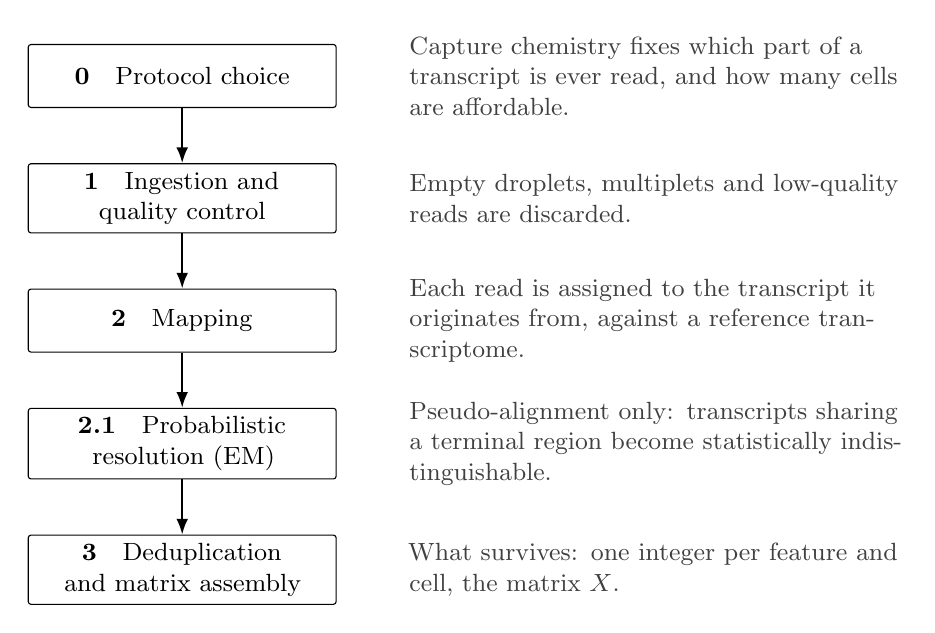
\begin{tikzpicture}[
  node distance=7mm,
  box/.style={draw, rounded corners=1pt, align=center, text width=3.7cm, minimum height=0.8cm, inner sep=3pt, font=\small},
  note/.style={align=left, text width=6.2cm, font=\footnotesize, text=black!75},
  ar/.style={-{Latex[length=2mm]}, thick}
]
\node[box] (p0) {\textbf{0}\quad Protocol choice};
\node[box, below=of p0] (p1) {\textbf{1}\quad Ingestion and quality control};
\node[box, below=of p1] (p2) {\textbf{2}\quad Mapping};
\node[box, below=of p2] (p3) {\textbf{2.1}\quad Probabilistic resolution (EM)};
\node[box, below=of p3] (p4) {\textbf{3}\quad Deduplication and matrix assembly};
\node[note, right=8mm of p0] (n0) {Capture chemistry fixes which part of a transcript is ever read, and how many cells are affordable.};
\node[note, right=8mm of p1] (n1) {Empty droplets, multiplets and low-quality reads are discarded.};
\node[note, right=8mm of p2] (n2) {Each read is assigned to the transcript it originates from, against a reference transcriptome.};
\node[note, right=8mm of p3] (n3) {Pseudo-alignment only: transcripts sharing a terminal region become statistically indistinguishable.};
\node[note, right=8mm of p4] (n4) {What survives: one integer per feature and cell, the matrix $X$.};
\draw[ar] (p0) -- (p1);
\draw[ar] (p1) -- (p2);
\draw[ar] (p2) -- (p3);
\draw[ar] (p3) -- (p4);
\end{tikzpicture}
\caption{The four phases of the preprocessing pipeline and the information each one removes. Phase~2.1 exists only on the pseudo-alignment route, where ambiguous reads must be distributed probabilistically; direct alignment resolves every read by its coordinates and skips it. The chemistry chosen in Phase~0 bounds every later stage, so the losses accumulate rather than cancel.}\label{fig:pipeline}
\end{figure}

\subsection{Phase 0: Choosing the Protocol}

The design of any \gls{scRnaSeq} analysis pipeline is inherently constrained by the physical protocol used for data generation. This experimental choice dictates the scale, resolution, and \gls{sparsity} of the resulting \gls{countMatrix}. Table~\ref{tab:protocols} compares the droplet protocol against plate-based methods.

\begin{table}[h]
\centering
\small
\setlength{\belowcaptionskip}{10pt}
\caption{The two dominant single-cell library chemistries. Per-cell depth and cost trade off against throughput; total reads per day are set by the sequencer, not the chemistry. All figures describe a single sequencing run. Values are order-of-magnitude, after Ding et al.\ \cite{ding2020systematic}.}\label{tab:protocols}
\begin{tabular}{lcc}
\toprule
 & \textbf{Plate (SMART-seq2)} & \textbf{Droplet (10x)} \\
\midrule
Library preparation & $\sim 2$ days for $96$ cells & $\sim 1$ day for $10^{4}$--$10^{5}$ cells \\
Cells per experiment & $10^{2}$--$10^{3}$ & $10^{4}$--$10^{5}$ \\
Reads per cell & $\sim 10^{6}$ & $\sim 10^{4}$ \\
Detected transcripts per cell & $\sim 10^{4}$--$10^{5}$ & $\sim 10^{3}$ \\
Reads per day & $\sim 10^{8}$--$10^{9}$ & $\sim 10^{8}$--$10^{9}$ \\
Coverage & full transcript & 3' terminus only \\
Reagent cost per cell & $\approx 10$--$100\times$ higher & baseline \\
\bottomrule
\end{tabular}
\end{table}

The widespread adoption of droplet protocols is ultimately driven by economics. While a plate-based experiment costs one to five dollars per cell, droplet encapsulation profiles cells for a few cents, allowing researchers to assay two to three orders of magnitude more cells on a fixed budget \cite{conte2024opportunities}. This trade-off between per-cell depth and cell quantity is highly advantageous for standard tasks like cell-type clustering, marker discovery, and differential gene expression. For these gene-level questions, the statistical power gained by averaging over thousands of cells overcomes the severe sparsity within individual cells. However, the loss of transcript coverage remains a fundamental limitation for \gls{isoform}-level analyses.

\subsection{Phase 1: Data Ingestion and Quality Control}

The first computational challenge in a single-cell pipeline is purely one of scale and structure. Sequencers output raw data in \gls{fastq} format, representing each read across four distinct lines: a coordinate identifier\defn{Read identifier}{A line beginning with \texttt{@} that names the read and records the instrument, flow cell and coordinates it came from.}, the nucleotide sequence\defn{Nucleotide sequence}{The read itself, a string of A, C, G and T bases in the order the sequencer read them.}, a separator\defn{Separator}{A line beginning with \texttt{+} that marks the end of the sequence and may repeat the identifier.}, and the corresponding Phred-scale quality scores\defn{Per-base quality score}{One character per sequenced base, encoding the probability that the base was called incorrectly on the Phred scale.}. For droplet-based chemistries such as the 10x Genomics platform, this raw sequence carries critical multiplexing metadata that must be carefully isolated before any biological analysis begins. Specifically, the sequencer must extract a \gls{cellBarcode} that maps the read back to its discrete cell of origin, and a \gls{umi}---a random tag attached prior to \gls{pcr} amplification used to track individual captured mRNA molecules.

Before the reads can be quantified, they must be cleaned. Tools such as cutadapt\defn{cutadapt}{A read-trimming tool that removes adapter sequences and low-quality bases.} or fastp\defn{fastp}{A fast all-in-one read preprocessor that performs adapter trimming, quality filtering and reporting in a single pass.} trim synthetic adapters, discard low-quality bases, and extract the barcode and UMI payloads, while heuristic filtering separates valid cell barcodes from empty droplets and multi-cell collisions (multiplets). The step is optional, and is skipped under two conditions. When a vendor pipeline such as Cell~Ranger has already trimmed adapters and corrected barcodes and UMIs, repeating the pass costs a full read of the FASTQ file without altering a base. When the mapper is read-structure-aware and UMI-aware, as alevin-fry and Salmon are, residual adapters fall outside the indexed $k$-mers and are never matched, so correction is left to the quantifier. Skipping is safe only under those guarantees: on untrimmed reads handled by a mapper that does not correct UMIs, adapters mis-assign reads and sequencing errors inflate the number of distinct UMIs. For plate-based chemistry no barcode or UMI exists to extract and adapter content is low, so trimming reduces to a quality filter.

Because quality control touches every single nucleotide exactly once, it acts as a highly parallelisable streaming operation strictly bound by the total read count, $R$, and the read length, $L$. The computational time complexity is entirely linear. The physical footprint, by contrast, is large. One uncompressed FASTQ record---a $100$\,bp read together with its identifier and quality line---occupies roughly $250$ bytes, so a droplet experiment of $R \sim 10^{9}$ reads, the order of magnitude considered here, holds $\sim 2.5 \times 10^{11}$ bytes, about $250$\,GB before compression. Modern multi-core trimmers sustain throughputs on the order of $10^{8}$ reads per minute, so this I/O-bound filtering resolves in a few hours on a single workstation.

\subsection{Phase 2: Mapping Algorithms (Alignment vs.\ Pseudo-Alignment)}\label{sec:pseudo-align}

Quantifying transcript expression requires mapping short sequencing reads back to their reference transcripts of origin. The computational workload is primarily driven by the total read count, $R = N \cdot M$. For the two datasets analysed in this thesis, $R$ is approximately $10^{8}$ to $10^{9}$, establishing $10^{9}$ reads as a baseline scale (though pooled multi-sample atlases can easily reach $10^{11}$ reads).

The mapping process is further defined by three variables: the number of annotated isoforms ($T \sim 10^5$), the average transcript length ($L_{avg} \approx 1500\text{ bp}$), and the sequenced read length ($L \approx 90\text{--}150\text{ bp}$). In a $3'$ droplet assay, Read~1 isolates the cell barcode and UMI, leaving only Read~2 to capture the actual transcript sequence ($L$).

Traditional alignment algorithms\defn{Read alignment}{Base-by-base mapping of a read to the reference, giving exact coordinates at high computational cost.} (e.g., BWA \cite{li2009bwa}, Bowtie2 \cite{langmead2012bowtie2}) map these sequences base-by-base to assign exact genomic coordinates, typically relying on a Burrows-Wheeler Transform\defn{Burrows-Wheeler Transform (BWT)}{A reversible text transform that allows fast substring search in a compressed reference index.} index. While building this index is a one-time operation scaling as $\mathcal{O}(T \cdot L_{avg})$, querying it is computationally expensive. Because the algorithm must accommodate sequencing errors and mutations, it uses a branch-and-bound search that scales logarithmically with the reference size. Consequently, the total query time becomes:
$$ \mathcal{O}(T \cdot L_{avg}) + \mathcal{O}(R \cdot L \log T) $$
For the billions of reads generated in a single-cell experiment, this error-tolerant sequence searching becomes a severe bottleneck, making exhaustive alignment prohibitively slow.

Modern transcriptomics tools like Salmon, alevin-fry, and kallisto \cite{patro2017salmon, bray2016near, he2022alevin} bypass this bottleneck through pseudo-alignment. This approach relies on a key insight: downstream single-cell quantification only requires identifying the source transcript, not its exact genomic coordinates. By discarding base-level alignment, pseudo-alignment replaces logarithmic sequence searches with constant-time hash table lookups.

This approach operates in two computational phases. First, index construction decomposes the reference transcriptome into a colored de Bruijn graph\defn{Colored de Bruijn graph}{A graph of overlapping $k$-mers in which each $k$-mer is coloured by the transcripts containing it, used as the pseudo-alignment index.} that maps short sequences of length $k$ ($k$-mers) to their parent transcripts. Rather than materialising every theoretically possible sequence, the index only stores the $k$-mers actually observed in the reference. This maintains a manageable spatial footprint of $\mathcal{O}(d)$ for $d$ distinct $k$-mers; for a mammalian transcriptome $d \sim 10^8$, far below the $4^{31}$ theoretically possible $k$-mers. Second, during the query phase, each read is split into overlapping $k$-mers (roughly $60$ to $120$ per read). The algorithm queries the hash table for each $k$-mer and intersects the results to rapidly identify an equivalence class\defn{Equivalence class}{The set of transcripts that could have produced a read, since all contain the read's $k$-mers.}---the set of reference transcripts compatible with that read.

Because this method shifts the core operation from sequence alignment to hash retrieval, the per-read query cost decouples entirely from the size of the reference transcriptome. The total execution time simplifies to:
$$ \mathcal{O}(T \cdot L_{avg}) + \mathcal{O}(R \cdot L) $$

The practical impact of this reduction is substantial. Using the baseline scale of $R \sim 10^{9}$ reads, $L \sim 10^{2}\text{ bp}$, and $T \sim 10^5$ (where $\log_2 T \approx 16.6$), traditional alignment's query phase requires approximately $1.7 \times 10^{12}$ operations. In contrast, pseudo-alignment requires roughly $1.0 \times 10^{11}$ operations. This $50$- to $100$-fold performance leap occurs because pseudo-alignment drops the asymptotic $\log_2 T$ factor and replaces expensive string matching with efficient hash lookups, ultimately reducing processing times from days to hours.

\subsubsection{Phase 2.1: Probabilistic Resolution via Expectation-Maximization}

Pseudo-alignment introduces a distinct computational challenge: multi-mapping reads\defn{Multi-mapping read}{A read compatible with more than one transcript because those transcripts share its sequence.}. These occur when a read's $k$-mers match multiple transcripts that share exonic sequences. If a read falls entirely within a shared exon, it carries no sequence information to identify its specific isoform of origin, prompting the pseudo-aligner to return a set of valid candidates rather than a single definitive transcript. This ambiguity is particularly severe in $3'$-biased protocols, where short reads exclusively capture the terminal region and frequently match every isoform sharing that terminal exon \cite{galfre2021cotan}.

Discarding these ambiguous reads is statistically unsound. Because they constitute the vast majority of alignments in $3'$-biased data, removing them would severely deplete the count matrix and artificially bias isoform proportions toward rare variants that happen to carry unique sequences. Instead, modern pseudo-aligners resolve this ambiguity by framing quantification as maximum-likelihood estimation over a generative model of the sequencing experiment \cite{patro2017salmon}.

In this model, each read fragment is assumed to be produced in two stages. First, a transcript $t$ is drawn with probability proportional to its abundance $\theta_t$. Second, a start position is drawn uniformly from the $\ell_t$ valid positions where a fragment of the observed length could begin. This admissible count, $\ell_t$, represents the transcript's \defn{Effective length}{The number of fragment start positions a transcript can generate; approximately its length minus the fragment length, plus one. It corrects for the fact that longer transcripts yield more fragments at equal abundance.}. Crucially, the true transcript of origin remains latent; the pseudo-aligner only reports the equivalence class $C_r$ \cite{bray2016near}. Marginalising over the unobserved origin yields the probability of observing that class under a given abundance vector:
$$ P(C_r \mid \theta) = \frac{\sum_{t \in C_r} \theta_t \, \ell_t}{\sum_{t'} \theta_{t'} \, \ell_{t'}} $$

Because the origin of each read is unobserved, this likelihood is optimised using the Expectation-Maximization (EM)\defn{Expectation-Maximization (EM)}{An iterative algorithm that estimates transcript abundances and resolves ambiguous read assignments jointly until they converge.} algorithm, which alternates between two phases until convergence. In the Expectation step (E-step)\defn{E-step / M-step}{The two alternating EM phases: distribute reads by the current abundance estimate (E), then re-estimate abundances (M).}, the current abundance estimate is used to compute the posterior probability that read $r$ originated from transcript $t$, given that it belongs to the class $C_r$:
$$ \hat{z}_{rt} = \frac{\theta_t \, \ell_t}{\sum_{t' \in C_r} \theta_{t'} \, \ell_{t'}} \quad \text{for } t \in C_r, $$
and $\hat{z}_{rt} = 0$ otherwise. The effective-length term $\ell_t$ is critical here: it accounts for the fact that a longer transcript contributes proportionally more fragments at equal abundance, ensuring $\hat{\theta}$ is not biased toward shorter isoforms. The algorithm then proceeds to the Maximization step (M-step), where each abundance is re-estimated as the total posterior weight assigned to its transcript:
$$ \theta_t \propto \sum_{r \,:\, t \in C_r} \hat{z}_{rt} $$
These values are subsequently normalised so that $\theta_t$ sums to exactly one across the transcriptome.

Two properties of this iteration influence the interpretation of the resulting counts. First, because each EM round is guaranteed not to decrease the log-likelihood, the estimates converge monotonically to a local optimum, though not necessarily a global one \cite{dempster1977maximum}. Since the likelihood surface is frequently flat or multimodal, implementations typically initialise $\theta$ uniformly and stop when the relative change in log-likelihood falls below a specified tolerance. Second, the model relies on a closed-world assumption: every read is assumed to originate from an annotated transcript. Consequently, incomplete references or unannotated isoforms propagate directly into $\hat{\theta}$. The resulting point estimate lacks intrinsic uncertainty, meaning downstream methods that require variance---such as the differential transcript usage (DTU) tools discussed later---must recover it by bootstrapping the quantification step \cite{love2018swimming}.

Computationally, because the EM updates run over equivalence classes rather than individual reads, the algorithm scales with the number of distinct classes. Tools like alevin-fry's parsimonious variant exploit this by collapsing transcripts that share identical $k$-mer sets into single groups, effectively performing gene-level quantification where isoform resolution is impossible \cite{he2022alevin}.

This collapsing behaviour highlights a fundamental identifiability limit inherent to $3'$ capture protocols. Consider two isoforms, $t$ and $t'$, of the same gene whose reads fall entirely into equivalence classes containing both---a common scenario when a shared terminal region covers their effective lengths. During the E-step, posterior weight is assigned solely through the ratio $\theta_t \ell_t / (\theta_t \ell_t + \theta_{t'} \ell_{t'})$. If $\ell_t \approx \ell_{t'}$, this ratio reduces to $\theta_t / (\theta_t + \theta_{t'})$. As a result, the likelihood depends on the two abundances only through their sum and remains flat along $\theta_t + \theta_{t'} = \text{constant}$. Every proportional split of abundances explains the observed reads equally well. This identifiability problem is bounded by the sequence divergence at the terminal region, not by the estimator, the reference, or sequencing depth; sequencing the same fragment more deeply cannot separate two transcripts that the fragment itself cannot distinguish. Consequently, transcript-level analyses of $3'$-biased data can only reliably recover isoform switches that differ at or near their $3'$ ends.

\subsection{Phase 3: Deduplication and Matrix Generation}

Once each read has been assigned to a transcript, the remaining task is to count molecules rather than reads. The protocol attaches a \gls{umi}---a short random sequence---to each captured molecule before amplification, so every read carries both a \gls{cellBarcode} identifying its cell and a UMI identifying its molecule. Because PCR copies inherit both tags, the reads descending from one molecule are indistinguishable duplicates, and collapsing each such group recovers the molecule counts that sequencing had inflated.

The collapse must be performed on barcode, UMI \emph{and} assigned transcript together. A UMI holds only a few random bases, so within one cell two unrelated molecules can share a UMI by chance; grouping on barcode and UMI alone would merge them, whereas including the transcript keeps them apart whenever they originate from different features.

The result is the expression count matrix $X$, whose entry $x_{fc}$ records the number of distinct molecules observed for feature $f$ in cell $c$. Amplification no longer distorts the counts, so the differences remaining between cells reflect biology and capture efficiency rather than how often each molecule happened to be copied.



\section{COTAN Framework}\label{sec:cotan-framework}

The transcript-level matrix $X$ produced above acts as the natural input for the statistical framework presented here, yet it simultaneously introduces the primary analytical difficulty: the shallow per-cell depth heavily imposed by the droplet hardware leaves the vast majority of its entries at zero. The COTAN framework, introduced by Galfr\`e et al.\ \cite{galfre2021cotan}, was specifically engineered to analyse this zero-heavy structure directly, and has since been logically extended to recover entire cell clusters purely from co-expression patterns \cite{galfre2026gene}. The following subsections formalise this sparsity and detail the contingency-table machinery COTAN employs to successfully bypass traditional density-based statistics.

\subsection{The Sparsity Problem}\label{sec:the-sparsity-problem}

Single-cell count matrices exhibit extreme structural sparsity. The disparity between the reference transcriptome and the yield of a single cell sets the scale: if $T \sim 10^5$ annotated isoforms sit in the reference while a single cell recovers only $T_{obs} \sim 10^3$ distinct transcripts, raw alignment space carries an initial zero rate of approximately $99\%$. Standard preprocessing pipelines subsequently filter out unexpressed or ultra-rare features, condensing the effective feature space to $T_{filtered} \approx 1.2 \times 10^4$--$2.3 \times 10^4$ viable transcripts, yet the observed zero rate typically remains between $70\%$ and $90\%$ \cite{galfre2021cotan}.

These zeros fall into two categories: biological zeros\defn{Biological zero}{A zero count reflecting genuine absence of a transcript in a cell, as opposed to a technical dropout.} (where the cell did not express the transcript) and technical \glspl{dropout} (where the molecule was present but failed to be captured). Because the cumulative efficiency of droplet capture, reverse transcription, and sequencing is only $10\%$ to $20\%$ \cite{jiang2022statistics}, technical dropouts dominate. Once recorded, both types of zeros are numerically identical in the count matrix and cannot be distinguished by count-based tests alone: a transcript that was truly absent and one that was merely missed leave the same mark \cite{sarkar2021separating}. Furthermore, the $3'$ terminus\footnote{\textbf{3' (three-prime) terminus} is the end of a transcript at which the poly-A tail is added; capture chemistry anchored here reads only the terminal fragment, not the transcript body.} \gls{tagBias} exacerbates this sparsity by collapsing distinct isoforms that share terminal exons into a single observational unit. That ambiguity, rather than the sparsity itself, is the fundamental statistical barrier for conventional tools designed for deep, dense \gls{bulkRnaSeq} data.

Applying standard density-based statistical methods to such sparse matrices introduces severe, compounding computational artifacts. Log-normalisation, which strictly involves adding a pseudo-count before logarithmic scaling, heavily distorts low-abundance measurements and artificially compresses legitimate zeros into spurious scaling patterns \cite{galfre2021cotan}. Standard linear or rank-based association measures, such as Pearson or Spearman correlations, fail entirely in this domain, as they inevitably end up measuring the coincidence of technical dropouts rather than identifying true regulatory co-expression \cite{galfre2021cotan}. Furthermore, attempting to artificially densify the matrix through heuristic imputation---specifically replacing zeros with smoothed estimates derived from neighbouring cells---frequently introduces fabricated correlations and severely compromises sensitive downstream signals \cite{galfre2021cotan}. To fundamentally circumvent these pitfalls, COTAN explicitly abandons imputation and variance-stabilising transformations entirely, choosing instead to evaluate the zeros as a direct signal through strict binary discretisation.

\subsection{Contingency Table Solution}

As stated, COTAN cleanly bypasses the flawed continuous count amplitudes by evaluating pairwise feature dependencies using asymptotic independence testing applied strictly to binary presence and absence states \cite{galfre2021cotan}. For any given feature pair $(f, f')$ across $N$ cells, the continuous counts are logically reduced to discrete indicator variables for each cell $c$:
$$ a_c = \mathbf{1}[x_{fc} > 0], \qquad b_c = \mathbf{1}[x_{f'c} > 0] $$
where $a_c$ marks whether feature $f$ is detected in cell $c$ and $b_c$ whether its partner $f'$ is. Letting the discrete states be indexed by $i, j \in \{0,1\}$, the framework constructs a comprehensive $2 \times 2$ \gls{contingencyTable} where $O_{ij}$ directly denotes the observed number of cells exhibiting state $a_c = i$ and $b_c = j$. The marginal totals for this specific table are defined as $\mathrm{Row}_i = \sum_j O_{ij}$ and $\mathrm{Col}_j = \sum_i O_{ij}$, mathematically constrained by the total cell count $\sum_i \mathrm{Row}_i = \sum_j \mathrm{Col}_j = N$. Under the standard null hypothesis of statistical independence, the expected cell count $E_{ij}$ is calculated directly as:
$$ E_{ij} = \frac{\mathrm{Row}_i \cdot \mathrm{Col}_j}{N} $$

Table~\ref{tab:contingency} lays the four counts out explicitly. The two diagonal cells hold cells in which the features are detected together ($O_{11}$) or neither is detected ($O_{00}$); the off-diagonal cells hold cells defining the difference between them, in which exactly one of the two is present. Co-expression resides in the tendency of the count to fall on a diagonal rather than on the anti-diagonal, and the expected value $E_{ij}$ above is what that count would be under the independence hypothesis.

\begin{table}[htbp]
\centering
\small
\setlength{\tabcolsep}{7pt}
\caption{The $2 \times 2$ contingency table built for a feature pair $(f, f')$ across $N$ cells. Entry $O_{ij}$ counts cells with $a_c = i$ and $b_c = j$; the margins are the feature's detection totals.}\label{tab:contingency}
\begin{tabular}{lccc}
\toprule
 & \textbf{$f'$ detected ($b_c = 1$)} & \textbf{$f'$ absent ($b_c = 0$)} & \textbf{Row total} \\
\midrule
$f$ detected ($a_c = 1$) & $O_{11}$ & $O_{10}$ & $\mathrm{Row}_1$ \\
$f$ absent ($a_c = 0$) & $O_{01}$ & $O_{00}$ & $\mathrm{Row}_0$ \\
\midrule
Column total & $\mathrm{Col}_1$ & $\mathrm{Col}_0$ & $N$ \\
\bottomrule
\end{tabular}
\end{table}
Deviation from this independent expectation is evaluated using Pearson's chi-squared statistic \cite{galfre2021cotan}:
$$ \chi^2 = \sum_{i \in \{0,1\}} \sum_{j \in \{0,1\}} \frac{(O_{ij} - E_{ij})^2}{E_{ij}} $$

The result is reported not as a statistic but as a single coefficient. COTAN defines the co-expression coefficient $C_{f,f'}$ by rescaling the deviation so that it lies in $(-1, 1)$ and, under the null hypothesis, satisfies $N\,C_{f,f'}^2 \sim \chi^2(1)$ over the $N$ cells of the table. The pairwise $p$-value, the quantity used for screening throughout this thesis, then follows directly:
$$ p_{f,f'} = P\!\left(\chi^2(1) > N\,C_{f,f'}^2\right) $$
A positive coefficient means the two features are detected together more often than independence predicts; a negative one means less often, which is the mutual exclusivity that Chapter~\ref{chap:methods} treats as the signal of interest.

One modification separates $C_{f,f'}$ from the textbook Phi coefficient of a $2 \times 2$ table, and it lies in the expectation rather than in the statistic. Taking $E_{ij}$ proportionally to the marginals, as above, assumes that every cell has the same chance of expressing a given feature. Cells differ widely in library size, so the cells that capture less RNA accumulate zeros across all features at once, and a proportional expectation would read that shared under-detection as co-expression and inflate the coefficient. COTAN therefore derives the expected co-occurrence from a model of the zeros themselves, calibrated per feature and per cell from the zeros actually observed; the reader is referred to the COTAN paper for the exact form of that model \cite{galfre2021cotan}. Co-expression is thus measured against how often two features' zeros were expected to coincide, not against their raw marginals.

The chi-squared approximation behind $p_{f,f'}$ is asymptotic in the number of cells, not in the counts, and the distinction matters here. With $N$ in the thousands the calibration is reliable for features detected in a reasonable fraction of cells, which covers most of a standard gene matrix. It degrades in the opposite regime, where a feature is rare enough that several expected cell counts $E_{ij}$ fall below about five; Pearson's statistic is then anti-conservative, and such a pair is best read as inconclusive rather than significant. Filtering cannot remove this effect for the rarest transcripts.

\subsection{Output Metrics}

The framework reduces the machinery above to three output metrics \cite{galfre2021cotan}.

The co-expression matrix $C$ captures the pairwise associations between features through the calculated coefficient $C_{f,f'}$. Within this matrix, positive values represent co-expression, whereas negative values indicate mutual exclusivity.

The \gls{gdi} is calculated from the co-expression matrix prior to any cellular clustering and functions as a per-feature measure of cluster specificity. For feature $i$ it takes the mean of the smallest $5\%$ of the feature's pairwise $p$-values, $\bar{p}_i$, and applies the transformation $\mathrm{gdi}_i = \ln(-\ln \bar{p}_i)$ to compress the distribution into an interpretable scale \cite{galfre2021cotan}. Features with constitutive expression form a uniform lower tail around a null median of roughly $1.305$. Conversely, features that vary across subpopulations produce very small $p$-values and rise above approximately $1.5$, which separates cell-type markers from housekeeping features.

Differential expression analysis (DEA) determines whether a single feature $f$ is statistically enriched within a specific cell cluster $S$. It applies the contingency-table structure to compare the presence or absence of feature $f$ against cells located inside versus outside cluster $S$, yielding the correlation coefficient $D_{f,S}$ on the bounded scale $(-1, 1)$. A positive $D_{f,S}$ reveals that the feature is detected more frequently inside the cluster, while a negative value signifies it is detected less often. Because all DEA coefficients share this standardized scale, the enrichment values can be directly compared across different features and clusters.

COTAN also provides functions for cell clustering, separate from these metrics but built on the GDI: a uniform-clustering step that groups cells into clusters whose gene expression is homogeneous, checked by ensuring no more than a small fraction of genes exceed a GDI threshold, followed by a merging step that collapses clusters which remain uniform when joined. DEA operates on whichever clusterization is supplied, so the two are connected but distinct capabilities.

\section{The Theoretical Basis of DTU in Sparse scRNA-seq}

\subsection{The Probabilistic Definition of a Switch}

Differential Gene Expression (\gls{deg}) and Differential Transcript Usage (\gls{dtu}) target fundamentally different mathematical properties of the transcriptome. DGE strictly measures overall changes in total, aggregated gene abundance between conditions; if $\theta_g$ represents the total absolute abundance of a parent gene $g$, DGE models shifts in $\theta_g$ directly. DTU, conversely, models the conditional probability of observing a specific transcript $t$ given that its parent gene is expressed. Let $\theta_t$ represent the absolute abundance of transcript $t$; the continuous relative proportion of that transcript is therefore $P(t \mid g) = \theta_t / \theta_g$. A theoretical isoform switch occurs when the conditional probability $P(t_1 \mid g)$ of one variant significantly increases between biological conditions or cellular states while $P(t_2 \mid g)$ simultaneously decreases, a regulatory shift that can occur entirely independently of any change in the total aggregated abundance $\theta_g$.

\subsection{Translating Continuous Proportions to Binary Sparsity}

Traditional bulk RNA-seq tools model the continuous proportion $P(t \mid g)$ directly, a statistical approach that relies on deep, junction-spanning coverage to provide stable density. In the extreme sparsity of droplet data (Section~\ref{sec:the-sparsity-problem}), a continuous proportional model breaks down. Because the cumulative efficiency of droplet capture and sequencing is exceedingly low, as an isoform's relative proportion drops, its already-low integer count is overwhelmingly pushed entirely into the zero state, registering as \gls{dropout}. Consequently, a continuous regulatory shift in biological proportions manifests mathematically in the single-cell count matrix as asymmetric binary presence and absence across cells.

\subsection{The Theoretical Limit of Observability}

The underlying pseudo-alignment quantification model imposes a strict theoretical boundary on which DTU events are mathematically identifiable from the matrix. As established in Section~\ref{sec:pseudo-align}, the pseudo-aligner maps sequences not to exact coordinates but to equivalence classes $C_r$, representing the set of all transcripts compatible with a given read. If two actively switching isoforms $t_1$ and $t_2$ differ strictly in their internal exonic structure but share identical sequences at their $3'$ terminus, all terminal reads generated by droplet protocols will invariably fall into an equivalence class containing both variants. During quantification, the Expectation-Maximization (EM) algorithm assigns posterior weights based on the length-adjusted ratio $\theta_{t_1} \ell_{t_1} / (\theta_{t_1} \ell_{t_1} + \theta_{t_2} \ell_{t_2})$. If their effective lengths are approximately equal ($\ell_{t_1} \approx \ell_{t_2}$), the likelihood surface remains entirely flat along the constraint $\theta_{t_1} + \theta_{t_2} = \text{constant}$. Every proportional split of abundances explains the observed terminal reads equally well, rendering the true $P(t \mid g)$ unidentifiable. Therefore, the framework is theoretically constrained: it can only successfully detect DTU events---such as alternative $3'$ terminus usage or terminal exon variation---where sufficient sequence divergence allows the short terminal fragments to map to distinct, informative equivalence classes.

\subsection{Mutual Exclusivity Signal}\label{sec:mutual-exclusivity}

Within the adapted COTAN framework, negative statistical associations---formally defined as \gls{mutualExclusivity}---between features serve as the foundational indicator of alternative usage patterns. When applied specifically to multiple isoforms of the exact same parent gene, this structural mutual exclusivity is biologically consistent with alternative splicing or \gls{isoformSwitch} events, wherein different cellular states preferentially express entirely distinct transcript variants.

However, mutual exclusivity in isolation is insufficient to prove a functional switch, since a strong negative association can also arise from sparse detection rather than from a real switch. One way to demonstrate the switch, consistent with the $P(t \mid g)$ definition, is bidirectional opposition: a cluster in which one isoform is preferred and another in which the preference flips to its partner. This confirms that different cell types genuinely use different isoforms, rather than leaving the exclusivity explainable by sparsity.
\chapter{Materials and Methods}\label{chap:methods}


Before walking through the workflow stages one by one, an overview of the whole is worth a glance: Figures~\ref{fig:overview} and~\ref{fig:overview-r} split it into two halves by the one artifact they share---an unfiltered isoform count matrix. The first half turns raw \gls{fastq} reads into transcript-level counts (Section~\ref{sec:pipeline}); the second takes that matrix, filters and cleans it, and runs the COTAN analysis and turns the counts into \gls{dtu} candidates (Sections~\ref{sec:data-filtering} and \ref{sec:methods-dtu-algorithm} onward).

Each half is implemented by a separate piece of code. The first half is driven by a custom Nextflow pipeline written for this thesis: it chains download, index, alignment and quantification around \texttt{nf-core/scrnaseq} (v4.1.0), runs on the cluster, and ends where the raw count matrix is written. The second half is driven by the \texttt{cotanisoform} R package together with config-driven analysis scripts, both written for this thesis; they consume that matrix, filter and clean it, and run COTAN to yield the \gls{dtu} candidates. The two halves therefore never share a runtime: the heavy sequencing work lives in Nextflow, the statistical work in R.


\usetikzlibrary{arrows.meta, positioning, decorations.pathreplacing}
\begingroup
\setlength{\textfloatsep}{2em plus 2pt minus 4pt}
\setlength{\floatsep}{1em plus 2pt minus 2pt}
\vspace{2em}
\begin{figure}[htbp]
    \centering
    \resizebox{\linewidth}{!}{%
    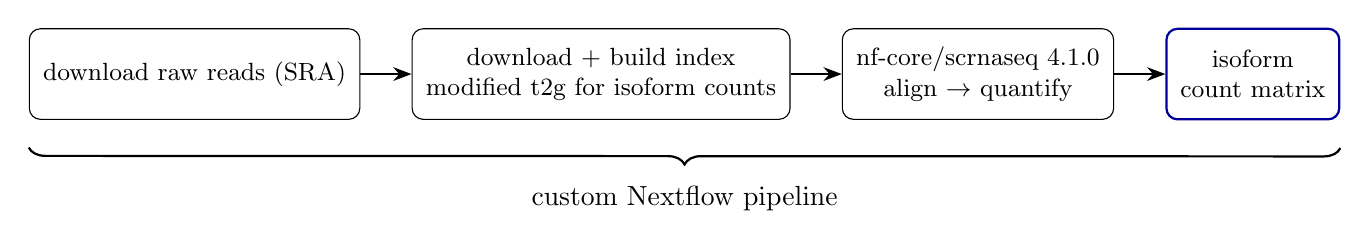
\begin{tikzpicture}[
        box/.style={draw, rounded corners, minimum height=1.15cm, inner sep=5pt, align=center, font=\footnotesize},
        arr/.style={-{Stealth}, thick},
        sep/.style={right=0.65cm of #1},
    ]
        \node[box] (reads) at (0,0) {download raw reads (SRA)};
        \node[box, sep=reads] (index) {download + build index\\modified t2g for isoform counts};
        \node[box, sep=index] (quant) {nf-core/scrnaseq 4.1.0\\align $\rightarrow$ quantify};
        \node[box, draw=blue!60!black, thick, sep=quant] (matrix) {isoform\\count matrix};

        \draw[arr] (reads) -- (index);
        \draw[arr] (index) -- (quant);
        \draw[arr] (quant) -- (matrix);

        \draw[thick, decorate, decoration={brace, amplitude=6pt, mirror}]
            ([yshift=-10pt]reads.south west) -- ([yshift=-10pt]matrix.south east)
            node[midway, below=10pt] {custom Nextflow pipeline};
    \end{tikzpicture}}
    \caption{Overview of the first half of the workflow: a custom Nextflow pipeline turns raw \gls{fastq} reads into an unfiltered isoform count matrix.}
    \label{fig:overview}
\end{figure}

\begin{figure}[htbp]
    \centering
    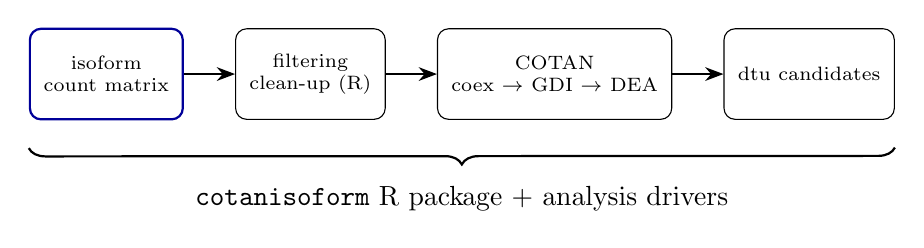
\begin{tikzpicture}[
        box/.style={draw, rounded corners, minimum height=1.15cm, inner sep=5pt, align=center, font=\scriptsize},
        arr/.style={{-{Stealth}}, thick},
        sep/.style={right=0.65cm of #1},
    ]
        \node[box, draw=blue!60!black, thick] (matrix) {isoform\\count matrix};
        \node[box, sep=matrix] (filter) {filtering\\clean-up (R)};
        \node[box, sep=filter] (cotan) {COTAN\\coex $\rightarrow$ GDI $\rightarrow$ DEA};
        \node[box, sep=cotan] (dtu) {\gls{dtu} candidates};

        \draw[arr] (matrix) -- (filter);
        \draw[arr] (filter) -- (cotan);
        \draw[arr] (cotan) -- (dtu);

        \draw[thick, decorate, decoration={brace, amplitude=6pt, mirror}]
            ([yshift=-10pt]matrix.south west) -- ([yshift=-10pt]dtu.south east)
            node[midway, below=10pt] {\texttt{cotanisoform} R package + analysis drivers};
    \end{tikzpicture}
    \caption{Overview of the second half of the workflow: the isoform count matrix is filtered, cleaned, and processed through COTAN's co-expression, GDI and DEA stages to yield the \gls{dtu} candidates.}
    \label{fig:overview-r}
\end{figure}
\endgroup

Table~\ref{tab:toolchain} records the tools and versions used in both halves, each with the section that justifies its choice.

\begin{table}[htbp]
    \caption{Tools used in this thesis: role, version, and the section justifying each choice.}\label{tab:toolchain}
    \vspace{0.5em}
    \small
    \setlength{\tabcolsep}{5pt}
    \begin{tabular}{@{}l l >{\raggedright\arraybackslash}p{8.5em} l@{}}
        \toprule
        \textbf{Tool} & \textbf{Version} & \textbf{Role} & \textbf{Justified in} \\
        \midrule
        Nextflow & 26.04.4 & Pipeline orchestration & \ref{sec:pipeline} \\
        nf-core/scrnaseq & 4.1.0 & Automates index $\rightarrow$ align $\rightarrow$ quantify & \ref{sec:pipeline} \\
        simpleaf & 0.24.1 quant.\,/\,0.24.0 index & Orchestrates alevin-fry + piscem & \ref{sec:pipeline} \\
        alevin-fry & --- & Quantification; EM assignment & \ref{sec:pipeline} \\
        piscem & --- & Index construction & \ref{sec:pipeline} \\
        sra-tools & --- & FASTQ download & \ref{sec:pipeline} \\
        Ensembl & release 102 & Reference annotation & \ref{sec:pipeline} \\
        R & 4.5.3 & Analysis layer & \ref{sec:data-filtering} \\
        COTAN & 2.13.1 (be93aa8) & Contingency, co-expression, DEA, DTU & \ref{sec:data-filtering} \\
        Seurat & 5.5.1 & Count-object container & \ref{sec:data-filtering} \\
        \bottomrule
    \end{tabular}
\end{table}

\section{Data Acquisition and Dataset Selection}

This study is based on two publicly available, droplet-based single-cell RNA-sequencing datasets: the Arigoni human cell-line mixture (GSE243665\cite{arigoni2024benchmark}) and the Ding mouse brain dataset (GSE132044\cite{ding2020systematic}). Both were obtained as raw \gls{fastq} reads alongside their genome annotations. They were selected after evaluating potential candidates against specific inclusion criteria, which are detailed below.

Candidate datasets were drawn from the curated collection at \url{https://seriph78.github.io/COTAN_Datasets_analysis/}, rather than searching the Gene Expression Omnibus (GEO)\defn{Gene Expression Omnibus (GEO)}{NCBI's public database of published gene-expression datasets. It stores raw and processed data for re-analysis.}\cite{barrett2013geo} ad hoc. Importantly, these datasets are pre-validated. Their prior use in COTAN's original benchmarking studies confirms their compatibility with the framework and ensures they are free of major technical artifacts.

A limitation of this collection is the absence of publicly available transcript-level count matrices for \gls{scRnaSeq} data. This reflects standard field practices rather than an omission. By default, most pipelines---including CellRanger\defn{CellRanger / Seurat}{Standard pipelines (10x CellRanger, Seurat) that quantify and analyse scRNA-seq data, defaulting to gene-level counts.}\cite{zheng2017massively} and the standard Seurat workflow\cite{hao2024seurat}---collapse data to \gls{gene}-level counts. While transcript quantification is possible using pseudo-alignment tools like Salmon\cite{patro2017salmon} or alevin-fry\cite{he2022alevin}, these steps are frequently bypassed. Furthermore, even when transcript-level analysis is performed, the data is typically aggregated back to the gene level prior to publication. Consequently, transcript matrices must be generated directly from the raw \gls{fastq} files.

That rebuild can be automated from scratch with the \texttt{nf-core/scrnaseq} pipeline\cite{ewels2020nfcore}, a containerised Nextflow workflow that chains indexing, alignment and quantification behind a single invocation.

That choice, however, narrows the field: \texttt{nf-core/scrnaseq} supports barcode-based protocols only, with the 10x Genomics\cite{zheng2017massively} chemistries, versions 2 and 3, as the supported family, so any dataset analysed here must come from that chemistry family. Of the COTAN datasets, only the Arigoni human cell-line mixture and the Ding mouse brain dataset satisfy both this chemistry requirement and the availability of published barcode lists --- the two datasets introduced above.

Those two are, in fact, a fortunate pairing. The Arigoni mixture is the strong-signal case: its cell lines are well separated and each carries a distinct isoform programme, and its GEO deposit supplies published barcode labels per line, so the detector runs against known groups and its calls can be checked against cell-type identity. The Ding cortex is the weak-signal case: heterogeneous tissue with gradual transitions and subtler contrasts, where no published labels exist, so it forces the computational-partitioning route and the cross-resolution validation. The pair therefore brackets the difficulty spectrum---a clean, discrete test and a noisy, continuous one---so that the candidates converging across both (Chapter~\ref{chap:results}) argue for a method that generalises rather than one fitted to a single favourable context.

\subsection*{Raw Read Download}\label{sec:download}

The raw input is not uniformly FASTQ. SRA stores 10x single-read runs as aligned BAM files rather than as reads, so the download path depends on each accession's layout. A layout check picks the route: paired-end runs are fetched as FASTQs via \texttt{prefetch} + \texttt{fasterq-dump}, whereas single-end 10x runs are fetched as the TenX BAM (\texttt{prefetch --type TenX}) and converted back to FASTQs with \texttt{bamtofastq}\cite{leinonen2011sra}. The Arigoni and Ding deposits are both 10x single-end runs, so both take the BAM-then-\texttt{bamtofastq} path.

Two operational choices keep the downloads tractable. They stage in RAM (\texttt{/dev/shm}) and never touch persistent disk, because each sample is tens of gigabytes---about 18~GB of BAM or 8~GB of zipped FASTQ. And concurrency is capped to stay within SRA's rate limits.

\section{Alignment, Quantification, and Feature Generation}\label{sec:pipeline}

\subsection*{Algorithm Selection: alevin-fry (simpleaf) vs.\ kallisto}

Quantifying transcripts from raw reads requires a choice between alignment-based and pseudo-alignment-based pipelines, and that choice propagates into the UMI handling and ambiguity resolution that downstream analysis depends on. Pseudo-alignment was preferred here for the reasons set out in Section~\ref{sec:pseudo-align}. Two pseudo-aligners dominate single-cell transcript quantification, each pairing a pseudo-alignment engine with a UMI-deduplication step: kallisto with bustools, and alevin-fry with its \texttt{simpleaf} orchestrator. Table~\ref{tab:pseudoalign-tools} compares their primary characteristics.

\begin{table}[htbp]
    \centering
    \caption{Comparison of scRNA-seq pseudo-alignment architectures.}\label{tab:pseudoalign-tools}
    \vspace{0.5em}
    \small
    \setlength{\tabcolsep}{6pt}
    \resizebox{\linewidth}{!}{%
    \begin{tabular}{lcc}
        \toprule
        \textbf{Feature} & \textbf{kallisto | bustools} & \textbf{alevin-fry (simpleaf)} \\
        \midrule
        Multi-mapping handling & Full compatible set & Minimal set (parsimony) \\
        \gls{umi} deduplication & Standard collapse & Directional error modelling \\
        Execution speed & Fast ($\sim$10 min per sample) & Very fast ($\sim$5 min per sample) \\
        nf-core integration & Available, non-standard & Native (v4.1.0) \\
        \bottomrule
    \end{tabular}}
\end{table}

The \texttt{simpleaf} framework\cite{he2023simpleaf} (v0.24.1 for quantification, v0.24.0 for the index build), which orchestrates \texttt{alevin-fry} for quantification and \texttt{piscem} for indexing, was selected for three reasons. Its UMI handling is superior, since single-cell data relies on \glspl{umi} to correct \gls{pcr} amplification bias and the alevin-fry error model distinguishes true UMIs from sequencing errors more reliably. For reads compatible with multiple transcripts, alevin-fry resolves the ambiguity by parsimony, searching for the minimal set of transcripts that explains each UMI rather than counting it against every compatible transcript, which suppresses spurious low-abundance counts that would bias the within-gene proportions that \gls{dtu} detection reads out. Finally, \defn{nf-core}{A community repository of standardised, peer-reviewed Nextflow analysis pipelines.}nf-core/scrnaseq (v4.1.0) supports \texttt{simpleaf} natively, with fewer configuration quirks than the kallisto alternatives.

The parsimony resolution matters. Assigning a UMI to the full set of transcripts it is compatible with leaks counts from an abundant isoform onto lowly-expressed isoforms sharing its sequence, biasing the within-gene proportions that \gls{dtu} detection reads out. \texttt{parsimony}\defn{parsimony}{An alevin-fry \gls{umi}-resolution mode that searches for the minimal set of transcripts explaining each UMI, suppressing spurious low-abundance counts.} instead builds a parsimony graph and finds the minimal set of transcripts that explains each UMI, so spurious low-abundance counts are suppressed and the estimated proportions are better identified. The resolution can leave fractional counts on ties, which are rounded to integers before COTAN ingests the matrix.

Because the downstream analysis operates on binary presence and absence rather than on the abundance point estimates, bootstrapped abundance variance was not part of this pipeline and is of limited relevance to zero-based detection: the rounded counts are discretised into detection indicators before the co-expression statistics are computed.

\subsection*{Index Modification for Transcript-Level Resolution}\label{sec:modification-process}

Standard alevin-fry\cite{he2022alevin} output collapses to gene level by default via transcript-to-gene mapping\defn{Transcript-to-gene (t2g) mapping}{A file pairing each transcript with its parent gene; replacing it with an identity mapping prevents gene-level collapse.}. To extract transcript counts, the index files were modified before alignment, following the identity-mapping route discussed in the \texttt{simpleaf} issue tracker\footnote{\url{https://github.com/COMBINE-lab/simpleaf/issues/115} (accessed 29 September 2026)}:

\begin{enumerate}
    \item \textbf{Identity mapping in \texttt{t2g\_3col.tsv}}: the standard mapping is replaced by a self-referential one, which prevents the final aggregation step that sums isoforms into genes.
{\small\begin{verbatim}
# Original: ENSMUST00000193814  ENSMUSG00000067548  # parent gene
# Modified: ENSMUST00000193814  ENSMUST00000193814  # itself
\end{verbatim}}

    \item \textbf{Removal of \texttt{gene\_id\_to\_name.tsv}}: the nf-core pipeline uses this file to map Ensembl gene identifiers to gene names during annotation. With the identity mapping in place the matrix rows are Ensembl \emph{transcript} identifiers, so the annotation step finds no gene IDs to match and halts. Removing \texttt{gene\_id\_to\_name.tsv} from the index trips a safety guard in alevin-fry: the annotation step checks for the file's presence and, finding it absent, skips the step. The guard does not itself know that annotation would halt on transcript IDs; the removal is deliberate, and it prevents that halt. The transcript counts were already written to disk, so they are kept and carried into the analysis.
\end{enumerate}

This modification is \textbf{reversible}: transcript-level quantification is a finer partition of the gene-level signal, so summing the transcript rows by gene using the retained \texttt{t2g} and \texttt{gene\_id\_to\_name} tables recovers a gene-level matrix directly, without rebuilding the index or re-aligning. This transcript-level route is an unsupported workaround, since alevin-fry is built for gene-level collapse and the identity-mapping modification is not an official mode. The gene-level matrix recovered by summing the transcript rows therefore matches a native gene-level run, except where the two resolutions assign ambiguous reads differently.

\subsection*{Reproducible Workflow Automation}

To make this workflow reproducible across datasets, it was automated with \textbf{Nextflow}\cite{ditommaso2017nextflow} (v26.04.4), a domain-specific language for computational pipelines that handles parallelization and checkpointing. This choice provides error handling, containerized dependencies, and standard configuration across datasets.

The custom automation script:

\begin{itemize}
    \item \textbf{Input}: a CSV samplesheet listing each sample and its SRA accessions\defn{Sequence Read Archive (SRA)}{NCBI's repository of raw sequencing data, accessed by identifiers such as SRR accessions.}, and a per-dataset configuration naming the genome assembly and species, the Ensembl release (102), the 10x chemistry, and the published barcode list. The pipeline downloads the reference FASTA and GTF\defn{GTF (Gene Transfer Format)}{An annotation file listing each gene's coordinates, exon structure, and transcript boundaries; used to build the transcriptome index.} from Ensembl itself, so a matching assembly name replaces a manual reference download. The configuration is not limited to these fields: it also carries options for the alignment mode, the index strategy, and other pipeline parameters, which are left at sensible defaults unless a dataset needs them.
    \item \textbf{Automated steps}:
    \begin{enumerate}
        \item Download the raw reads (Section~\ref{sec:download}): FASTQs for paired-end runs, BAM-then-\texttt{bamtofastq} for 10x single-end runs.
        \item Download the Ensembl reference and build the gene-level \texttt{piscem} index.
        \item If transcript-level output is requested, create a cheated transcript-level copy of that index by applying the identity-mapping modification.
        \item Execute nf-core/scrnaseq (v4.1.0) with \texttt{simpleaf}.
        \item Produce the raw count matrix and its metadata.
    \end{enumerate}
    \item \textbf{Availability}: the complete workflow, including configuration files and test cases, is available at \url{https://github.com/ldelitala/sc-isoform-cotan}.
\end{itemize}

The workflow ends at the count matrix. Quality filtering and the COTAN analysis are performed afterwards in the R analysis layer (R 4.5.3), keeping the two concerns separate.

Adapter trimming is omitted deliberately rather than by oversight. The 10x read structure places the barcode and UMI in a fixed header segment, and \texttt{simpleaf} resolves that geometry internally with a UMI-aware error model, discarding residual adapter $k$-mers because they match no indexed sequence. A separate \texttt{fastp} pass would therefore reread the entire FASTQ file for no change in the count matrix. Quality control at the barcode level still runs: \texttt{simpleaf} applies empty-droplet detection to the quantification output, and cells are further restricted to the high-quality barcode sets published with each dataset (Section~\ref{sec:data-filtering}).

\section{Data Processing and Quality Control}\label{sec:data-filtering}

Before the COTAN object is built, the Seurat assay's counts are rounded to the nearest integer and explicit zeros are dropped, since COTAN ingests integer counts; the fractional parsimony-em assignments never enter the framework directly. The COTAN object is then initialised from this Seurat object, and all subsequent filtering operates on it. From this point onward Seurat is no longer used; the rest of the workflow operates exclusively on the COTAN object.

\subsection*{Cell-Level Filtering}

Cells were filtered using metadata from the original GEO publications. The Arigoni dataset (GSE243665\cite{arigoni2024benchmark}) and the Ding dataset (GSE132044\cite{ding2020systematic}) both provide lists of cells that passed their quality control thresholds, and restricting the analysis to those known-good barcodes avoids a second QC pipeline that could introduce inconsistencies. Published studies typically filter on a minimum UMI count per cell, which removes empty droplets; a maximum mitochondrial read percentage\defn{Mitochondrial read percentage}{The fraction of a cell's reads coming from mitochondrial genes; abnormally high values flag dying or damaged cells.}, which removes dying cells; and a gene detection threshold, since cells with too few detected genes may be doublets or otherwise low quality. Reusing their filtering ensures comparability and reduces methodological drift.

The unfiltered matrices are dominated by empty droplets; restricting to the barcodes the original studies report as passing their quality control yields the cell counts. Concretely, the passing-cell barcode lists were loaded into the COTAN object as a \texttt{passed\_QC} condition using the package's \texttt{flag\_valid\_cells\_from\-\_tsv()}, and the object was then subset with \texttt{filter\_cotan\_by\-\_condition()} to keep only cells flagged as passing; the per-cell-line Arigoni lists were combined first. Both functions are part of the \texttt{cotanisoform} R package\cite{ldelitala2026scisoform}, built on top of COTAN's object model.

\subsection*{Feature-Level Filtering}

Feature filtering ran in the R analysis layer (R 4.5.3) with COTAN (v2.13.1, commit \texttt{be93aa8}). Two filters act on the transcript set. First, \texttt{filter\_spliced\_transcripts()} keeps only spliced transcripts by matching the Ensembl feature names against a prefix (\textasciicircum\texttt{ENST} for human, \textasciicircum\texttt{ENSMUST} for mouse) and discarding the rest, then drops the cells that are left with no surviving feature. COTAN's framework\cite{galfre2021cotan} targets mature mRNA, and unspliced pre-mRNA has different statistical properties that can confound \gls{coexpression} analysis, so this restriction to spliced features both removes noise and shrinks the matrix. Second, \texttt{clean\_cotan\_data()} wraps COTAN's \texttt{clean()} routine with its default cutoffs: a transcript is kept only if it is expressed in at least 0.3\% of cells (\texttt{cellsCutoff}=0.003) and a cell only if it detects at least 0.2\% of the retained features (\texttt{genesCutoff}=0.002)---fractional cutoffs far stricter than a fixed count, because isoform-level detection is so sparse that an absolute threshold would admit thousands of near-empty rows. With \texttt{drop\_fully\_expressed} enabled, the few transcripts expressed in nearly every cell are physically removed as well.

These choices prioritize quality over quantity. Smaller matrices mean faster computation and cleaner signal---important when running expensive contingency table calculations across all feature pairs.

\subsection*{Statistical Estimation and the GDI}

With the filtered transcript matrix in the COTAN object, the framework's parameters are estimated and its statistics computed. The per-feature and per-cell expression probabilities $\lambda$ and $\nu$ are calibrated from the observed zeros, the pairwise co-expression coefficient $C_{f,f'}$ and its $p$-value are calculated for every feature pair, and the \gls{gdi} is derived from those $p$-values as the per-feature mean of the smallest $5\%$---the theory is laid out in Section~\ref{sec:cotan-framework}. The pipeline executes all of this in one step (\texttt{03\_calc.R}) and renders the resulting GDI into a diagnostic plot (\texttt{04\_gdi.R}) over a dataset-specific marker panel. This is the stage that turns the filtered counts into the co-expression structure the partition in the next section reads out of; without it, clustering would have nothing to group cells by.

\section{Population Partitioning and Validation}

Differential transcript usage is a contrast between groups of cells: an isoform switch surfaces only when the cells carrying one variant can be set against the cells carrying the other. The partition of cells fixes what the detector is able to see, and the two datasets reach that partition along different routes.

\subsection*{Ground-Truth vs.\ Computational Partitioning}

The Arigoni human cell-line dataset arrives already divided: its GEO deposit distributes one barcode list per constituent cell line and for the PBMCs, so those published labels serve directly as the groups the detector compares.

The Ding mouse cortex dataset arrives with no such labels. Its cells are grouped from the matrix itself with COTAN's hierarchical uniform clustering\defn{Hierarchical uniform clustering}{COTAN's procedure that recursively splits cells by co-expression dissimilarity, then merges statistically indistinguishable clusters.}. Cell-to-cell dissimilarity is read from the co-expression patterns, clusters are split until each becomes homogeneous, and neighbours the statistics cannot separate are merged. Run on transcript counts, the procedure returns a set of uniform clusters and a small noisy remainder---the cells whose expression matches no group closely enough to claim them. Those clusters are a hypothesis, not a verdict: COTAN was designed and validated on gene-level matrices, and this thesis is its first application at isoform level, so nothing guarantees the co-expression statistics still hold on transcripts.

\subsection*{Cross-Resolution Validation}

To give the transcript partition something to be measured against, the same cells were clustered a second time on gene counts: the official Ding gene matrix, cleaned with COTAN's standard \texttt{clean()} and clustered with parameters identical to the transcript run. Gene-level clustering is the established use of COTAN; over a denser feature set it stands as an independent reference partition rather than a cheaper substitute. The two partitions are then compared over their common cells by a confusion matrix\defn{Confusion matrix}{A table of cluster-label agreement between two clustering runs, revealing systematic splitting and merging.}, and the detector is run twice over the same transcript matrix, once with the transcript clusters and once with the gene-derived clusters standing in as ground truth, so that an event surviving both is a signal no choice of partition can manufacture. 
\section{The DTU Detection Algorithm}\label{sec:methods-dtu-algorithm}

The detector bypasses pseudo-bulk aggregation and instead reuses COTAN's gene-level machinery---the contingency table, the \gls{coexpression} coefficient, and the differential-expression contrast---applied at transcript resolution, so that a mutually exclusive isoform pair is recognised by the same independence test that already copes with sparsity\cite{galfre2021cotan}. The biological justification for the two filters is given in Section~\ref{sec:mutual-exclusivity}. For every gene with $k \ge 2$ detected isoforms, the procedure is:

\begin{enumerate}
    \item \textbf{\gls{mutualExclusivity} screening}: for every possible pair of isoforms $(A, B)$ within the gene:
    \begin{itemize}
        \item Read the \gls{coexpression} coefficient $C_{A,B}$ already computed for every feature pair in the estimation stage (Section~\ref{sec:data-filtering}), where it derives from the $2 \times 2$ \gls{contingencyTable} of presence and absence across cells\cite{galfre2021cotan} (Section~\ref{sec:cotan-framework}).
        \item Retain pairs with a negative $C_{A,B}$ and a $p$-value\defn{p-value}{The probability of observing an association this strong if the features were truly independent.} $< 0.05$.
    \end{itemize}

    \item \textbf{Contrast calculation}: for each significant pair, the differential enrichment is a vector over the partition's clusters,
    \begin{equation}
        \Delta_i = D_{A,i} - D_{B,i}, \qquad i \in \mathcal{P},
    \end{equation}
    where $D_{f,i}$ is COTAN's differential expression coefficient for feature $f$ in cluster $i$ (Section~\ref{sec:cotan-framework}) and $\mathcal{P}$ is the set of clusters in the partition. Each term $D_{f,i}$ lies in $(-1,1)$ because it is a correlation coefficient read from the $2 \times 2$ contingency table of feature presence against cluster membership, and such a coefficient is bounded to $(-1,1)$ by construction; the difference $\Delta_i$ therefore lies in $(-2,2)$, so the contrast is bounded and comparable across genes and clusters.

    \item \textbf{Bidirectional thresholding}: retain pairs that switch, which requires opposition in both directions:
    \begin{itemize}
        \item At least one cluster with $\Delta > \tau$.
        \item At least one different cluster with $\Delta < -\tau$.
        \item \defn{$\tau$ (contrast threshold)}{The minimum absolute DEA contrast between two isoforms required to count a cluster toward a switch.} $\tau$ is calibrated per dataset in the section that follows.
    \end{itemize}
\end{enumerate}

The algorithm outputs a list of gene-isoform pairs with evidence for cluster-specific differential usage, ranked by statistical significance and effect size ($|\Delta|$).

\section{Calibrating the Switch Threshold \texorpdfstring{($\tau$)}{(tau)}}\label{sec:tuning-tau}

The contrast threshold $\tau$ controls the balance between sensitivity and specificity: high values yield few confident calls but risk missing subtle switches; low values capture more events but increase false positives.

A tuning script was developed to study how the threshold affects the candidate set. It varies $\tau$ in fine steps across a range such as $0.02$ to $0.5$ (step $0.02$ for the Arigoni run, $0.01$ over $0.01$--$0.3$ for the Ding run), counts the detected DTU events at each threshold, plots the relationship between $\tau$ and the number of significant pairs, and suggests thresholds that yield biologically reasonable candidate counts, typically $20$--$100$ events for validation feasibility.

\chapter{Results and Discussion}\label{chap:results}

This chapter presents the findings from applying transcript-level COTAN to scRNA-seq data. It begins with quality assessment (GDI clustering validation) and a comparison of gene-level and transcript-level structure, before presenting the main contribution: DTU detection results across the human and mouse datasets. Each section builds toward answering whether sparse 3'-biased data can support isoform-switch discovery using contingency-table statistics.

\section{Dataset Quality Assessment via GDI}

Before DTU calls can be interpreted, the clustering must be shown to capture biological structure rather than technical noise. The Global Differentiation Index (GDI), defined in Section~\ref{sec:cotan-framework}, provides this validation.

\subsection*{Transcript-level Clustering Quality}\label{sec:gdi-transcript}

Figure~\ref{fig:gditranscript} shows the GDI plot for the mouse dataset clustered on transcript counts. Each point represents a cell, colored by its assigned cluster (11 uniform clusters total). The clear spatial separation indicates that transcript-level co-expression patterns distinguish distinct cellular populations.

Key observations from this visualization:
\begin{itemize}
    \item Cluster boundaries are well-defined with minimal overlap, suggesting robust isoform-based signatures.
    \item High-GDI genes (marker candidates) show selective enrichment in specific clusters rather than uniform expression.
    \item The noisy remainder cells (not assigned to any cluster) form a tight central cloud; these were filtered out from downstream DTU analysis.
\end{itemize}


This confirms that transcript-level data contains sufficient signal for meaningful clustering, despite sparsity and 3'-bias constraints.

\begin{figure}[htbp]
    \centering
    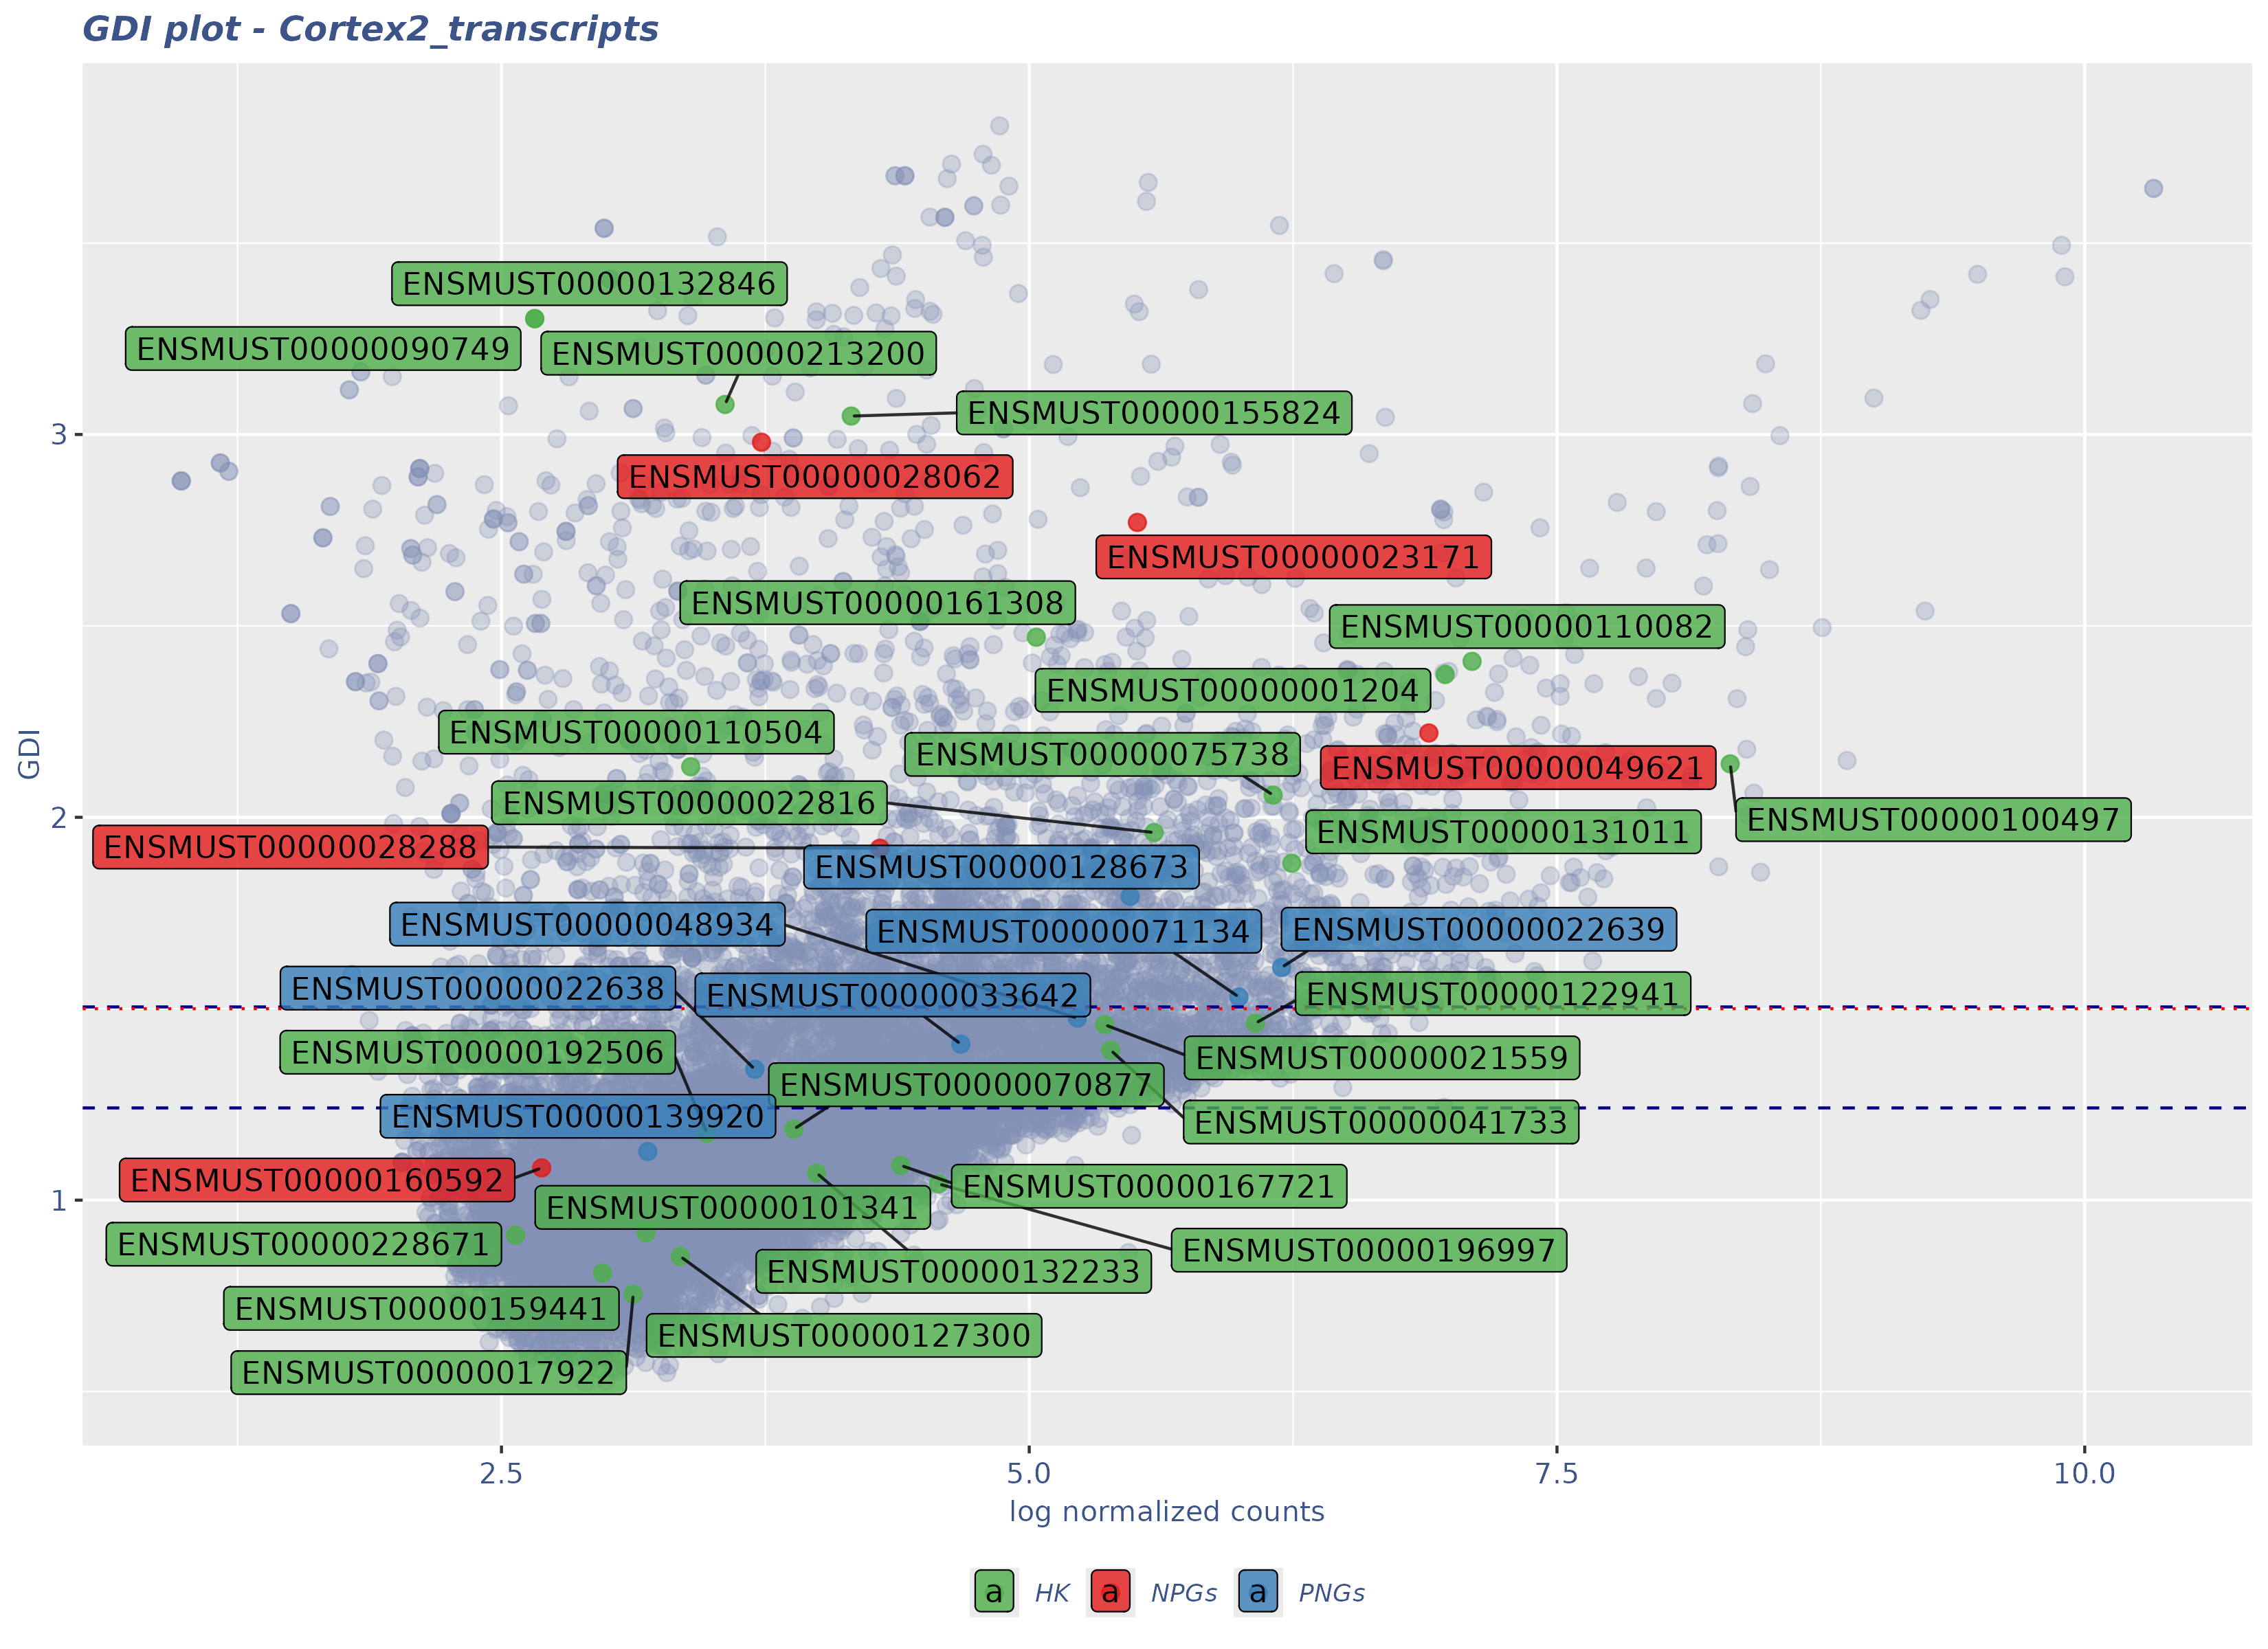
\includegraphics[width=0.8\textwidth]{GDI_transcript_plot_markers.png}
    \caption{GDI plot of the mouse dataset clustered on transcript-level counts, coloured by the 11 uniform clusters.}
    \label{fig:gditranscript}
\end{figure}

\subsection*{Gene vs Transcript Structure Comparison}

Figure~\ref{fig:gdi_genes} shows the same cells clustered using standard gene counts (15 clusters). The gene run reads the independent GEO gene matrix---28,692 features against the transcript matrix's 12,848---so its larger cluster count reflects the denser matrix, not a finer gene-level resolution.

\begin{figure}[htbp]
    \centering
    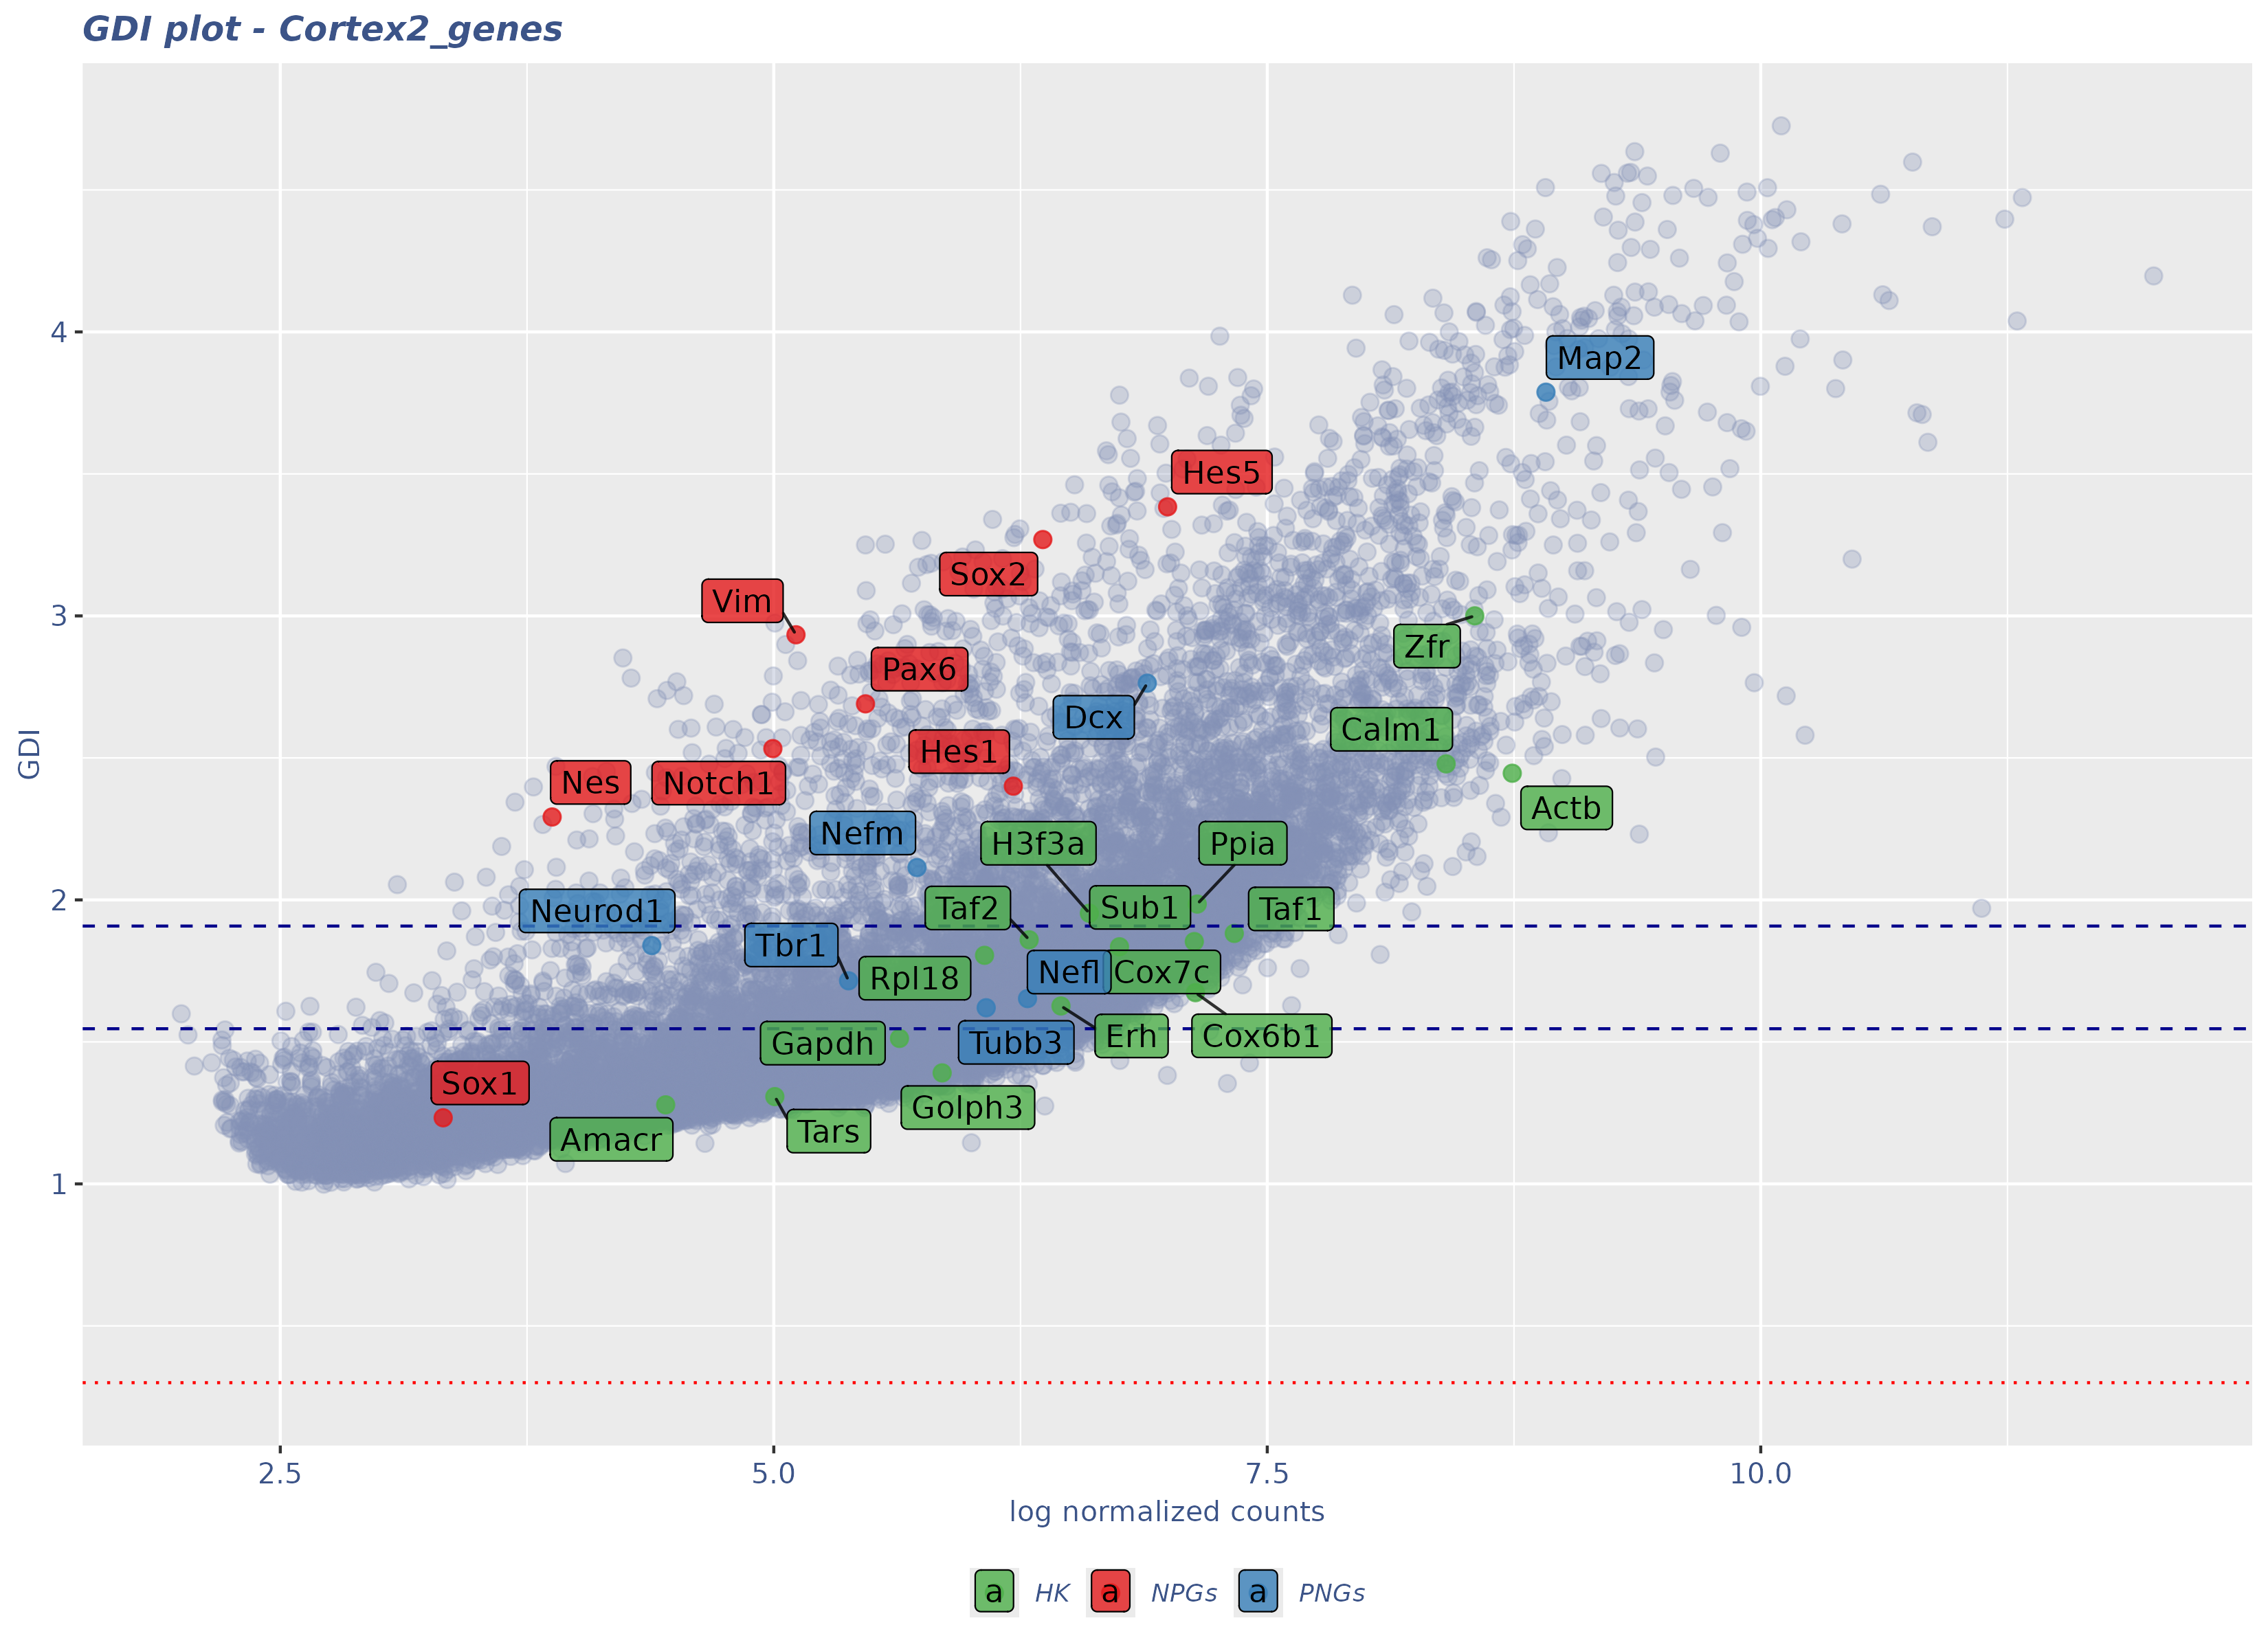
\includegraphics[width=0.8\textwidth]{GDI_genes_plot_markers.png}
    \caption{GDI plot of the same cells clustered on gene-level counts, yielding 15 clusters.}
    \label{fig:gdi_genes}
\end{figure}

These GDI analyses establish that both clustering approaches capture real biological signal, but with different sensitivity to cellular substructure. The main question is whether this structural difference translates into distinct DTU detection.

\section{Clustering Comparison: Gene vs Transcript Level}\label{sec:clustering-comparison}

To quantify how gene and transcript clustering diverge, a confusion matrix was constructed across 4,077 common cells present in both analyses.

\begin{figure}[htbp]
    \centering
    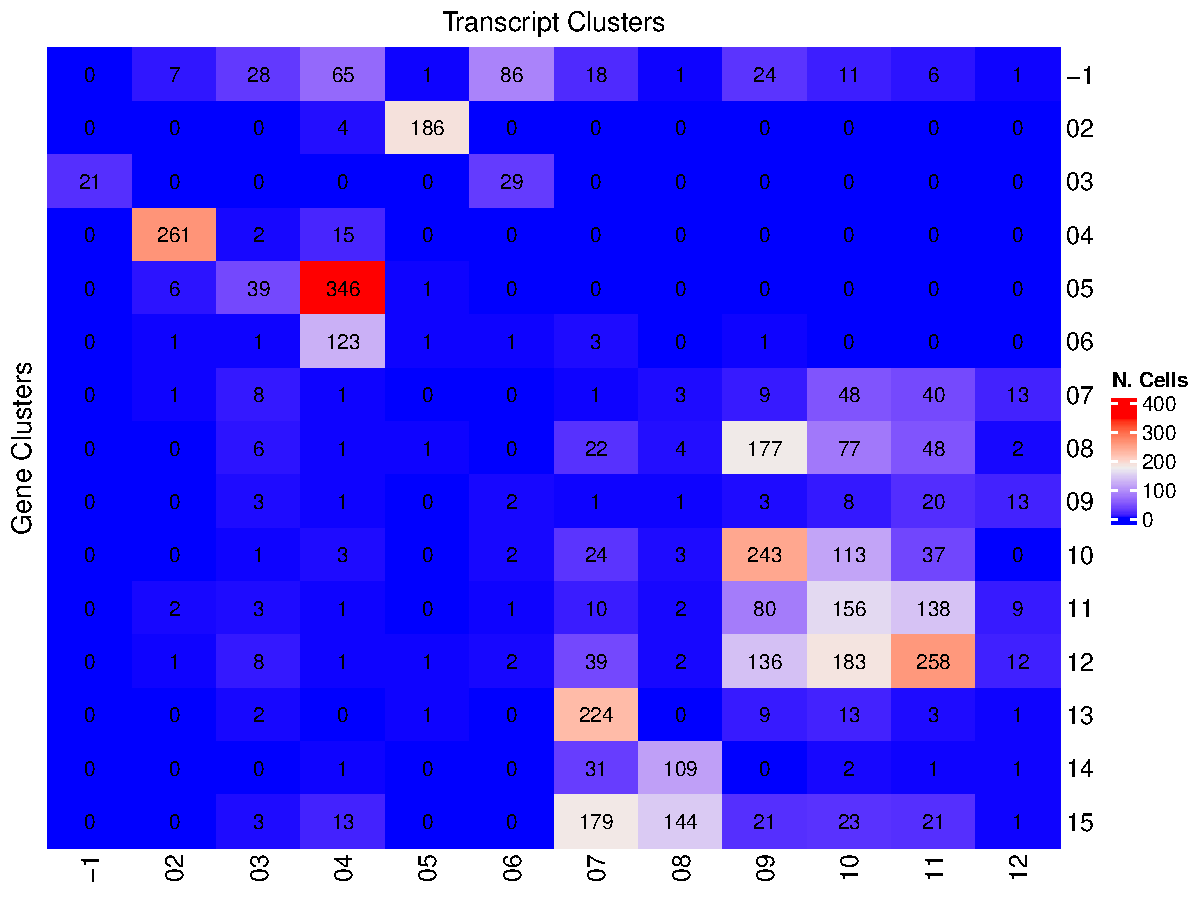
\includegraphics[width=0.8\textwidth]{heatmap_genes_vs_transcripts.pdf}
    \caption{Confusion matrix comparing transcript-level (11 clusters) and gene-level (15 clusters) assignments for the 4,077 common cells of the mouse dataset.}
    \label{fig:confusion-matrix}
\end{figure}

Figure~\ref{fig:confusion-matrix} shows the confusion matrix heatmap. Several patterns emerge:
\begin{itemize}
    \item \textbf{Diagonal dominance}: Most cells receive consistent assignments across both methods, validating that neither approach produces random clusters.
    
    \item \textbf{Systematic splitting}: Several transcript-level clusters correspond to sub-regions of single gene-level clusters. For example, transcript cluster 4 splits from the broader gene cluster 7, suggesting isoform variation within what appears homogeneous at gene resolution.
    
    \item \textbf{Selective merging}: Conversely, some adjacent transcript clusters merge in gene analysis, indicating that their differences rely on isoform-specific expression patterns rather than overall transcriptional activity.
\end{itemize}

The interpretation: across the two runs the counts differ (11 against 15) because the partitions come from different matrices---the transcript matrix is a sparser, feature-filtered view, the gene matrix a denser GEO count set---so the totals are not a resolution ranking. What the confusion matrix actually shows is agreement in the large and divergence in the particular: the dominant diagonal confirms both partitions recover the same broad populations, while the local splits and merges mark where isoform information changes the grouping. That is precisely the regime where DTU detection should add value---if isoform switches distinguish cell states that genes alone cannot separate, then transcript-aware methods capture biologically relevant signals.

However, this raises a critical question: whether the detected DTU events hold across clustering strategies, or depend entirely on how cells are partitioned. The robustness analysis below answers it.

\section{Core Finding: DTU Detection Results}\label{sec:dtu-results}
The algorithm from Section~\ref{sec:methods-dtu-algorithm} was applied to both human and mouse datasets, filtering for mutually exclusive isoform pairs with bidirectional cluster preference (threshold $\tau$ as specified). The results show that contingency-table statistics can recover within-gene exclusivity patterns even in sparse 3'-biased data.

\subsection*{Human Dataset Findings (Arigoni)}\label{sec:results-human}

The human cell line mixture provided ground-truth validation through known biology. Of the 4958 genes carrying at least two detected transcripts, 430 retain at least one significant mutually exclusive pair\footnote{Counted by \texttt{extract\_dtu\_candidates()} and recorded in the run log (\texttt{results/arrigoni/logs/}); the exported \texttt{dtu\_candidates.csv} holds only the 21 survivors.}, yet after the bidirectional contrast threshold $\tau = 0.2$ only 21 candidates survive, across just 9 genes. That collapse from 430 to 9 is the algorithm working as designed: mutual exclusivity alone admits hundreds of pairs, but only a handful also flip their enrichment between clusters, and it is this second condition---a pair must be preferred in one cell type and disfavoured in another---that separates a genuine switch from a statistical curiosity.

The surviving candidates cohere into a single story. TPM1, the strongest call, is a tropomyosin whose isoforms oppose each other across the cell lines: one isoform is enriched in PC9 and DV90 while the other dominates A549 and HCC78, a reciprocal preference that reads as cell-type-specific cytoskeletal tuning. Alongside it sit the ribosomal proteins RPL10 and RPS24, whose unexpected DTU signal points toward cell-type-specific translation regulation---consistent with the heterogeneity of ribosomal composition underlying specialised translation \cite{xue2012specialized}. The two themes are biologically distinct but converge in method: in both cases a single gene carries two isoforms that the same cell types use in opposite directions, and it is that convergence, not any single gene, that validates the detector. The final list is small precisely because the algorithm demands both \gls{mutualExclusivity} and a bidirectional contrast, and that conservative design is what lets nine genes carry the whole human result.

\subsection*{Mouse Dataset Findings (Ding)}\label{sec:results-mouse}

For mouse brain tissue a lower threshold, $\tau = 0.05$, was applied, and the balance shifts: only 14 genes carry significant pairs, yet 46 candidates survive across 8 genes. The inversion is itself informative---fewer initial pairs but more survivors means mouse cortex switches are gradual rather than sharp, so a relaxed threshold admits many weak but real transitions that the strict human cutoff would have discarded.

The candidates trace an arc across the tissue. Meg3, a long non-coding RNA\defn{Long non-coding RNA (lncRNA)}{A long RNA molecule that does not encode a protein but regulates gene expression, splicing, and development.} with a documented role in neuronal differentiation, switches along the differentiation trajectory itself: isoform A dominates early progenitor clusters while isoform B is enriched in differentiated neurons---a transition that tracks a continuous gradient rather than a binary state. Malat1, another highly conserved lncRNA involved in splicing regulation, shows the same cluster-specific preference, consistent with the alternative 3$'$ isoform usage documented for this locus \cite{ghanam2023malat1}. The two lncRNAs are neighbours in function---both non-coding, both switching with differentiation---and together they anchor the mouse result in established biology. The arc then turns inward: Srrm2 encodes a core spliceosome\defn{Spliceosome}{The molecular machine that removes introns and joins exons during splicing.} component, and its own DTU suggests feedback regulation, alternative splicing of splicing factors being a known mechanism for tuning isoform landscapes across cell states. Finally, Ttc14, a novel candidate with no prior DTU literature, requires \gls{orthogonalValidation} to confirm its biological significance---and its presence is a reminder that the method also surfaces calls no published study has anticipated.

\subsection*{Robustness Analysis: Shared vs Exclusive Events}\label{sec:robustness}

DTU detection was re-run using gene-derived cluster labels on the same transcript matrix, and the resulting event lists were compared across both clustering strategies. Both partitionings returned the same total, 46 DTU pairs; their composition differed:
\begin{itemize}
    \item \textbf{Shared events}: Majority of pairs detected by both methods, including Meg3 and Malat1---these represent strong signals surviving regardless of partitioning scheme.
    
    \item \textbf{Transcript-exclusive (3 pairs)}: Srrm2 and Ttc14 isoform switches appeared only with transcript-derived clusters. These likely reflect subtle transitions requiring fine-grained population resolution to detect.

    \item \textbf{Gene-exclusive (4 pairs)}: Snrnp70, Lrrc7, Zfp941, and a specific Meg3 pair detected only using gene-level clustering. These may represent weaker signals that benefit from aggregated statistical power.
\end{itemize}

The interpretation:
\begin{enumerate}
    \item Strongest DTU signals (high effect size) survive both approaches---validating the algorithm's core functionality.
    
    \item Subtle switches depend on clustering resolution: transcript-level captures isoform-specific states; gene-level provides power for low-abundance transcripts.
    
    \item Neither approach dominates universally. Researchers should consider their biological question when choosing---fine-grained substructure vs statistical robustness.
\end{enumerate}

This robustness analysis confirms that while the strongest signals are cluster-agnostic, subtle isoform switches reveal themselves only under appropriate partitioning schemes. The choice of clustering strategy is not merely technical---it shapes which biology becomes visible.

\subsection*{Threshold Sensitivity: The Tau Sweep}\label{sec:tau-sweep}

The candidate count depends on the contrast threshold $\tau$. To make the choice principled rather than arbitrary, the analysis re-runs the DTU extraction over a fine grid of $\tau$ values (0.005 to 0.3 at step 0.005) and records, at each threshold, the number of accepted events, the unique genes behind them, and how many survive the strictest threshold that still yields at least ten events (the robust core).

Two properties of the sweep matter for interpretation. First, the event count is monotone decreasing in $\tau$---a sanity check that the extraction responds predictably to the threshold. Second, the fraction of accepted events belonging to the robust core (\texttt{frac\_in\_core}) rises toward one as $\tau$ approaches the core threshold; a plateau in this fraction marks the point where further relaxation adds only weak, non-core switches.

Figure~\ref{fig:tau-sweep} maps that search across a landscape of thresholds. The bulk of significant pairs descends like a long, smooth slope---from 2006 at $\tau = 0.005$ to 21 at $\tau = 0.2$---a nearly featureless gradient that reflects the homogeneous cell-line mixture: every isoform pair carries some reciprocal contrast, so the terrain is a dense and continuous spectrum with no natural break. On such a slope any single threshold looks arbitrary, and this is exactly the trap the sweep is built to expose. As the eye climbs the landscape a highland finally appears: at $\tau = 0.25$ ten events, all belonging to the robust core, hold flat through $\tau = 0.26$---a genuine plateau, ground stable enough to stand on rather than a point on the slope. The published threshold $\tau = 0.2$ reproduces the 21 reported candidates and sits just below that highland, so the human result is anchored at the edge of stable ground rather than lost somewhere on the tail. The mouse terrain is different: it descends in steps, 46 events at $\tau = 0.05$ holding at 41 and 36 across wide intervals, because heterogeneous tissue is dominated by a few high-contrast switches with a sparse tail---so its plateaus are broad ledges, not a single summit.

\begin{figure}[htbp]
    \centering
    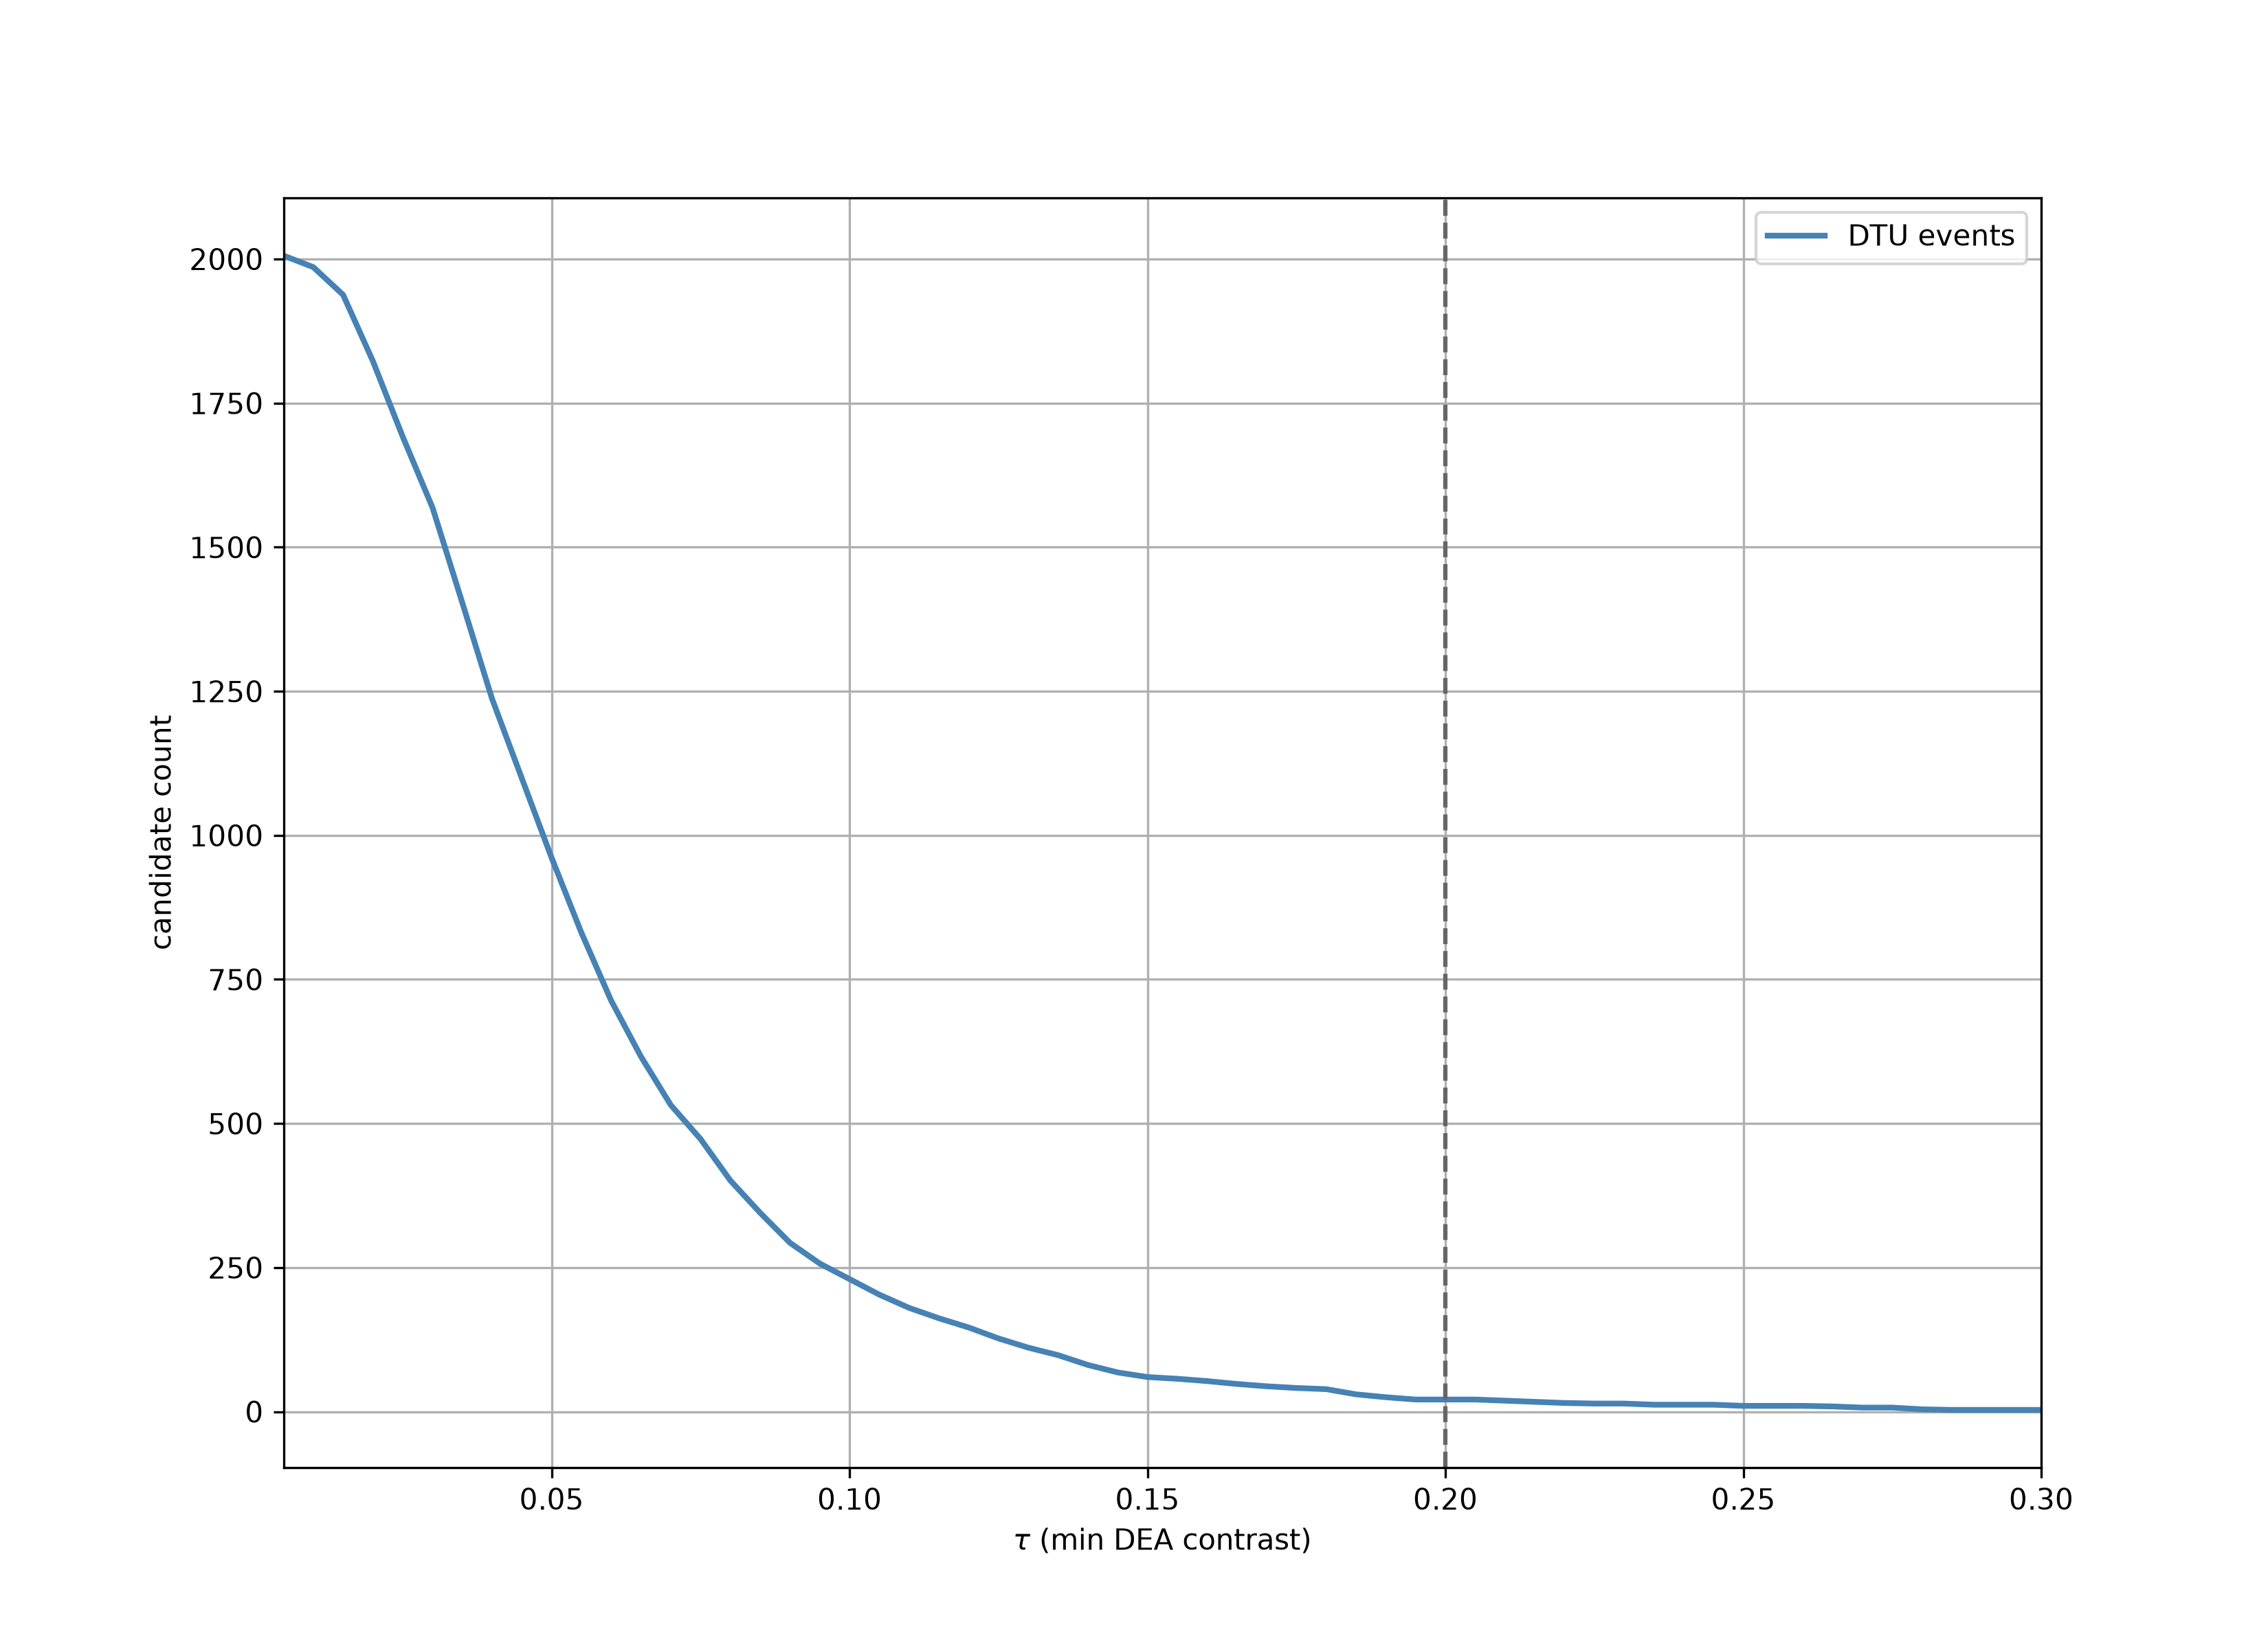
\includegraphics[width=0.8\textwidth]{arrigoni_tau_sweep.png}
    \caption{Tau sensitivity sweep for the human dataset: DTU events (blue) and robust-core events (orange) versus the minimum DEA contrast threshold $\tau$. A stable plateau appears at $\tau = 0.25$ with a ten-event core; the published $\tau = 0.2$ (dashed) reproduces the 21 reported candidates.}
    \label{fig:tau-sweep}
\end{figure}

The plateau provides an empirical anchor for $\tau$: the reported thresholds (0.2 human, 0.05 mouse) were chosen within or adjacent to stable regions, so the final candidate lists are not an artifact of a single fragile threshold value. The sweep does not, however, replace a permutation-based null distribution; it remains an internal-consistency check on how the accepted set changes with the threshold.

\section{Discussion}\label{sec:discussion}

These findings are now set within their broader methodological and biological context.

\subsection*{Key Findings Interpretation}

Two conclusions follow from these results. The top candidates (Meg3, Malat1, TPM1) align with documented biology---lncRNA switching in neurogenesis and ribosomal protein regulation---which indicates that the algorithm recovers genuine signal rather than technical artifacts. Convergence across a human cell line mixture and mouse brain tissue further indicates that the method holds under different biological contexts rather than a single favourable case study.

\subsection*{Limitations and Caveats}

Despite encouraging results, several constraints temper interpretation:
\begin{itemize}
    \item \textbf{3'-bias invisibility}: Alternative splicing events occurring in transcript mid-regions remain undetectable when only \gls{threePrimeEnd}s are sequenced. The DTU candidates found here represent a subset---those where isoforms differ at their terminal exons or 3' ends.

    \item \textbf{EM rounding effects}: Fractional EM assignments were rounded to integers for COTAN compatibility (Section~\ref{sec:data-filtering}). Low-abundance isoforms with small fractional counts may be distorted by this discretization, potentially introducing false negatives or altered contrast values.

    \item \textbf{Threshold sensitivity}: The choice of $\tau$ lacks formal statistical grounding. The tau sweep (Section~\ref{sec:tau-sweep}) anchors the threshold empirically at a stable plateau, but a permutation-based null distribution would still provide calibrated $p$-values rather than a consistency-based choice.

    \item \textbf{Lack of orthogonal validation}: Without long-read sequencing or targeted RT-PCR\defn{RT-PCR}{Reverse-transcription polymerase chain reaction: a lab technique that experimentally confirms whether a specific isoform is present, used as an orthogonal check on computational DTU calls.} confirmation, false positive rates remain estimated from internal consistency (shared vs exclusive events) rather than ground truth.

This is a limitation common to computational DTU studies but remains critical for biological claims.
\end{itemize}

\subsection*{Future Directions: Extending COTAN for Transcript Analysis}

The framework established here opens several avenues for methodological extension:
\begin{enumerate}
    \item \textbf{Integration with long-read data}: Combining short-read depth (thousands of cells) with PacBio/Nanopore\defn{Long-read sequencing (PacBio, Oxford Nanopore)}{Sequencing technologies that produce full-length transcript reads, giving complete isoform annotation unavailable from short 3'-biased reads.} isoform annotation would anchor DTU calls in complete transcript sequences.

This hybrid approach could validate computational predictions while scaling to population-level sample sizes.

    \item \textbf{Trajectory-aware analysis}: Current clustering assumes discrete cell populations, but differentiation is continuous. Modeling isoform proportions along pseudotime\defn{Pseudotime}{A one-dimensional ordering of cells along a continuous developmental or differentiation trajectory, capturing gradual transitions rather than discrete populations.} trajectories (e.g., using COTAN's framework adapted for regression rather than categorical comparison) could reveal dynamic switching patterns during transitions.

    \item \textbf{Allele-specific expression extension}: COTAN's contingency table approach naturally extends to phased variants. Detecting allele-biased isoform usage would connect regulatory genetics (eQTLs, sQTLs)\defn{eQTL / sQTL}{Genomic variants that measurably affect gene expression (eQTL) or splicing/isoform usage (sQTL); linking them to single-cell isoform switches connects population genetics with regulation.} to splicing outcomes in single cells---bridging population genomics with transcript regulation.

    \item \textbf{Benchmarking against bulk DTU tools}: Systematic comparison with rMATS, SUPPA2, and DRIMSeq \cite{love2018swimming, draper2025selecting} on matched pseudo-bulks would contextualize sensitivity and specificity. This benchmark could identify regimes where single-cell methods add unique value versus when aggregation suffices.
\end{enumerate}

These extensions remain beyond the scope of this thesis, but they indicate that the framework admits further adaptation as new data types and biological questions emerge.

\chapter{Conclusions}

While $3'$-biased droplet protocols strip away the internal transcript structure usually required for isoform analysis, this thesis demonstrates that some \gls{dtu} can still be reliably detected. By extending COTAN's sparsity-robust contingency-table framework to the transcript level, this work successfully recovered within-gene exclusivity patterns directly from sparse, terminal read counts.

\section{Summary of Findings}

Before extracting \gls{dtu} events, it was imperative to establish that the extreme sparsity inherent to $3'$-biased droplet data did not obscure the underlying biological signal. The analysis demonstrated that the transcript-level \gls{gdi} distribution successfully preserved enough differential variance to separate distinct cellular populations. Furthermore, transcript-level clustering recovered fine-grained cellular substructures that were entirely masked under standard gene-level aggregation partitions.

Applied to the two distinct single-cell datasets, the adapted contingency-table framework successfully returned detectable signals in both. In the human cell line mixture, the algorithm initially identified 430 genes exhibiting mutually exclusive isoform usage; after enforcing a rigorous bidirectional contrast filter, 21 high-confidence candidates survived. Similarly, in the highly heterogeneous mouse cortical tissue, 41 candidate switches passed the established lower contrast threshold in the transcript-derived partition (38 in the gene-derived one).

Crucially, the strongest DTU calls output by the pipeline---such as TPM1 in the human cell mixture, alongside Meg3 and Malat1 in the mouse cortex---are highly consistent with documented isoform biology \cite{ghanam2023malat1, xue2012specialized}. To ensure these findings were robust rather than methodological artifacts, the candidates were cross-validated against an alternative clustering strategy. The majority of the top isoform switches survived this swap, demonstrating that the detected structural mutual exclusivity represents a genuine regulatory signal that does not depend on any specific partitioning scheme.

\section{Broader Implications}

This work has implications across three domains:

\textbf{For computational genomics}: The success of contingency-table statistics at transcript resolution demonstrates that sparsity can be modelled directly rather than overcome (Section~\ref{sec:cotan-framework}). This philosophy may extend to other single-cell challenges---allele-specific expression, chromatin accessibility peak co-occurrence, and multi-modal integration.

\textbf{For isoform biology}: Detecting DTU in $3'$-biased data opens new analysis opportunities for existing large-scale datasets (e.g., Human Cell Atlas, Tabula Sapiens\defn{Human Cell Atlas / Tabula Sapiens}{Large international reference atlases of single-cell transcriptomes across human tissues, relied on 3'-biased droplet data and were therefore closed to isoform-level questions.}) that were previously closed to isoform-level questions. While sensitivity is limited compared to full-length protocols, the trade-off between cell numbers and coverage may favor droplet methods when statistical power from thousands of cells outweighs per-cell depth.

\textbf{For COTAN framework development}: This thesis validates that COTAN's core design principles, set out in Section~\ref{sec:cotan-framework}, generalize beyond gene-level analysis. Future extensions to other single-cell modalities (ATAC-seq\defn{ATAC-seq}{Assay for Transposase-Accessible Chromatin: maps genome regions where chromatin is open, indicating regulatory activity.} peak co-occurrence, protein abundance correlations in CITE-seq\defn{CITE-seq}{A protocol that simultaneously measures RNA and surface proteins in the same single cells, enabling multi-modal analysis.}) appear feasible.

\section{What This Work Leaves Behind}

Beyond the findings, this thesis leaves a set of reusable artefacts, published together in the public repository that accompanies it.

\textbf{A quantification pipeline.} The Nextflow pipeline (Section~\ref{sec:pipeline}) automates the path from raw reads to a count matrix, offering both the gene-level and the transcript-level index. Its steps run separately, so a re-run from an existing index does not repeat the download.

\textbf{An analysis library.} The \texttt{cotanisoform} R package collects the whole analysis path into documented functions: reading a count matrix, adapting it to COTAN, running the COTAN steps, extracting DTU candidates, and comparing runs. It can be installed and used on any single-cell dataset, independently of the two datasets studied here, and its logging layer lets a long run report its own progress and failures in one consistent trace.

\textbf{A reproducible analysis layer.} The driver scripts reproduce the complete analysis of a dataset from a single configuration file, one per dataset and feature level, so each reported table can be regenerated without interactive input.

\textbf{Documentation and reference outputs.} The repository documents the method and the parameters behind each published table, and it stores the published results themselves---the DTU candidate tables, tau-sweep and \gls{gdi} plots, and the run logs---under \texttt{results/}, one directory per dataset.

\section{Limitations and Future Work}

The constraints on these results---$3'$-bias invisibility, the absence of orthogonal validation, the heuristic threshold $\tau$, and EM rounding---are set out together with the directions they open in Section~\ref{sec:discussion}. The same underlying trade-off governs all four: sensitivity is bought with cells rather than coverage, so the value of the method grows as datasets do.

The framework established in this thesis opens several methodological extensions beyond the two datasets studied here:

\textbf{Integration with long-read data:} Combining short-read depth (thousands of cells) with PacBio/Nanopore\defn{Long-read sequencing (PacBio, Oxford Nanopore)}{Sequencing technologies that produce full-length transcript reads, giving complete isoform annotation unavailable from short 3'-biased reads.} isoform annotation would anchor DTU calls in complete transcript sequences. This hybrid approach could validate computational predictions while scaling to population-level sample sizes.

\textbf{Trajectory-aware analysis:} Current clustering assumes discrete cell populations, but differentiation is continuous. Modeling isoform proportions along pseudotime\defn{Pseudotime}{A one-dimensional ordering of cells along a continuous developmental or differentiation trajectory, capturing gradual transitions rather than discrete populations.} trajectories (e.g., using COTAN's framework adapted for regression rather than categorical comparison) could reveal dynamic switching patterns during transitions. Such an extension requires datasets suited to trajectory inference; the Ding samples were not, as the original paper states \cite{ding2020systematic}.

\textbf{Allele-specific expression extension:} COTAN's contingency table approach naturally extends to phased variants. Detecting allele-biased isoform usage would connect regulatory genetics (eQTLs, sQTLs)\defn{eQTL / sQTL}{Genomic variants that measurably affect gene expression (eQTL) or splicing/isoform usage (sQTL); linking them to single-cell isoform switches connects population genetics with regulation.} to splicing outcomes in single cells---bridging population genomics with transcript regulation.

\textbf{Benchmarking against bulk DTU tools:} Systematic comparison with rMATS, SUPPA2, and DRIMSeq \cite{love2018swimming, draper2025selecting} on matched pseudo-bulks would contextualize sensitivity and specificity. This benchmark could identify regimes where single-cell methods add unique value versus when aggregation suffices.

On the computational side, the pipeline and the analysis remain two halves joined at the count matrix: the Nextflow workflow ends at the filtered matrix, and the R analysis is started separately. Folding the analysis into the workflow as one further step would let a single run cover the path from raw accessions to DTU candidates, which is the main engineering direction this work leaves open.

A newer quantifier points the same way, but at a coarser grain than the EM step used here. SCALPEL\cite{ake2025scalpel} is a complete Nextflow pipeline that would substitute the whole quantification half of this work, from raw reads to a transcript matrix. Where it diverges from this thesis is at quantification itself: instead of an identity transcript-to-gene index resolved by alevin-fry's EM, SCALPEL filters internal-priming artefacts out of the aligned reads and builds an APA-aware isoform-level matrix (Section~\ref{sec:pipeline}). Its authors report higher sensitivity and specificity than existing tools on synthetic data, and predictions that agree with other tools and survive experimental validation on real data \cite{ake2025scalpel}. In future work, its transcript matrix would be fed into COTAN exactly as the matrix built here is, testing whether the downstream DTU calls sharpen---the contingency-table analysis would stay unchanged, and SCALPEL would simply supply a sharper, APA-aware input. That COTAN output would in turn be compared against SCALPEL's own differential-isoform-usage table, providing an independent DTU caller as an orthogonal cross-check on the contingency-table calls.

Bootstrapped quantification variance is a second extension. Abundance-based DTU tools recover the uncertainty of the EM point estimates by bootstrapping, but the contingency-table statistics used here operate on binary presence and absence, so the variance of those point estimates is of limited relevance to the reported calls. It still matters at the margin, where an estimate error near the detection threshold can flip a cell's detection state; recovering the variance by bootstrapping the quantification step would let a future analysis quantify that edge. It is left as future work rather than included here.

\section*{Final Remarks}

This thesis demonstrates that transcript-level COTAN can reveal regulatory programs hidden to gene-centric analyses, and that a contingency-table approach to sparse data respects the measurement process rather than imposing transformations designed for dense, normally distributed data. The framework established here---methodological rigour, computational reproducibility and alignment with known isoform switches---provides a foundation for that future work, which still requires orthogonal validation and the complementary technologies set out in Section~\ref{sec:discussion}. Whether applied to neurogenesis, cancer evolution, or developmental biology, the core question remains: \textit{which transcripts are cells expressing, and how does that choice change across conditions?}

% Bibliography (global, after all chapters)
\cleardoublepage
\addcontentsline{toc}{chapter}{Bibliography}
\bibliographystyle{unsrt}
\bibliography{bib/riferimenti}

% Appendix (optional)
\appendix
\chapter{Supplementary Data}
\section{Complete DTU Results (Arigoni and Ding Datasets)}

The tables below list every reported event. The same data are available as CSV in the public repository, so a reader can re-derive or re-filter them.

% --- TABELLA 1: ARRIGONI ---
\begin{landscape}
\begingroup
\footnotesize
\setlength{\tabcolsep}{4.5pt}
\begin{longtable}{@{} l l l >{\raggedright\arraybackslash}p{3.4cm} >{\raggedright\arraybackslash}p{3.4cm} r r r r @{}}
\caption{Significant DTU events in the human dataset (Arigoni 2024), including cluster enrichment and maximum contrasts.\label{tab:arrigoni_landscape}}\\
\toprule
\textbf{Gene} & \textbf{Tr.~A} & \textbf{Tr.~B} & \textbf{Clusters A} & \textbf{Clusters B} & \textbf{$\Delta$ A} & \textbf{$\Delta$ B} & \textbf{COEX} & \textbf{$p$-value} \\
\midrule
\endfirsthead
\toprule
\textbf{Gene} & \textbf{Tr.~A} & \textbf{Tr.~B} & \textbf{Clusters A} & \textbf{Clusters B} & \textbf{$\Delta$ A} & \textbf{$\Delta$ B} & \textbf{COEX} & \textbf{$p$-value} \\
\midrule
\endhead
\midrule
\multicolumn{9}{r}{\textit{Continued on next page}} \\
\endfoot
\bottomrule
\endlastfoot
TPM1   & ENST00000334895 & ENST00000358278 & DV90, HCC78, HTB178 & A549, CCL-185-IG & 0.33 & 0.61 & $-0.101$ & $7.72 \times 10^{-67}$ \\
RPL10  & ENST00000406022 & ENST00000458500 & A549 & HCC78, PC9 & 0.22 & 0.46 & $-0.086$ & $2.78 \times 10^{-49}$ \\
RPL10  & ENST00000458500 & ENST00000491035 & HCC78, PC9 & A549, PBMCs & 0.46 & 0.25 & $-0.084$ & $6.41 \times 10^{-47}$ \\
TPM1   & ENST00000404484 & ENST00000651344 & HCC78, HTB178 & A549, CCL-185-IG & 0.27 & 0.37 & $-0.074$ & $1.15 \times 10^{-36}$ \\
TPM1   & ENST00000317516 & ENST00000651344 & HCC78, HTB178 & A549, CCL-185-IG & 0.28 & 0.36 & $-0.068$ & $4.41 \times 10^{-31}$ \\
RPS24  & ENST00000360830 & ENST00000465692 & DV90, HCC78 & CCL-185-IG, HTB178, PBMCs & 0.28 & 0.30 & $-0.051$ & $1.76 \times 10^{-18}$ \\
TPM1   & ENST00000288398 & ENST00000334895 & A549, CCL-185-IG & HTB178 & 0.30 & 0.21 & $-0.047$ & $1.13 \times 10^{-15}$ \\
TPM1   & ENST00000560959 & ENST00000651344 & HCC78, HTB178 & A549, CCL-185-IG & 0.22 & 0.32 & $-0.044$ & $8.17 \times 10^{-14}$ \\
RPS24  & ENST00000360830 & ENST00000482069 & DV90, HCC78 & CCL-185-IG, HTB178, PBMCs & 0.28 & 0.28 & $-0.040$ & $8.15 \times 10^{-12}$ \\
TPM1   & ENST00000334895 & ENST00000651344 & DV90, HCC78, HTB178 & A549, CCL-185-IG & 0.28 & 0.44 & $-0.040$ & $8.76 \times 10^{-12}$ \\
DSTN   & ENST00000449141 & ENST00000474024 & HTB178 & CCL-185-IG & 0.28 & 0.22 & $-0.039$ & $3.70 \times 10^{-11}$ \\
SAT1   & ENST00000379253 & ENST00000462639 & A549 & PC9 & 0.26 & 0.27 & $-0.038$ & $6.62 \times 10^{-11}$ \\
TPM4   & ENST00000645471 & ENST00000646974 & CCL-185-IG & HCC78 & 0.32 & 0.39 & $-0.034$ & $5.27 \times 10^{-09}$ \\
SAT1   & ENST00000379251 & ENST00000462639 & A549 & PC9 & 0.22 & 0.21 & $-0.031$ & $7.47 \times 10^{-08}$ \\
SAT1   & ENST00000379270 & ENST00000487713 & A549 & PC9 & 0.25 & 0.25 & $-0.031$ & $9.35 \times 10^{-08}$ \\
RPL35A & ENST00000429437 & ENST00000642387 & PC9 & PBMCs & 0.21 & 0.22 & $-0.031$ & $1.26 \times 10^{-07}$ \\
TPM1   & ENST00000558544 & ENST00000651344 & HCC78, HTB178 & A549, CCL-185-IG & 0.23 & 0.33 & $-0.019$ & $1.04 \times 10^{-03}$ \\
TPM1   & ENST00000358278 & ENST00000558868 & A549, CCL-185-IG & CRL5868, DV90, HCC78, HTB178 & 0.52 & 0.27 & $-0.018$ & $1.96 \times 10^{-03}$ \\
SNHG5  & ENST00000654795 & ENST00000664396 & CCL-185-IG & PC9 & 0.23 & 0.28 & $-0.018$ & $2.37 \times 10^{-03}$ \\
RPS8   & ENST00000372209 & ENST00000485390 & PC9 & PBMCs & 0.21 & 0.29 & $-0.017$ & $4.19 \times 10^{-03}$ \\
TPM1   & ENST00000317516 & ENST00000358278 & DV90, HCC78, HTB178 & A549, CCL-185-IG & 0.33 & 0.54 & $-0.012$ & $4.03 \times 10^{-02}$ \\
\end{longtable}
\endgroup
\end{landscape}


% --- TABELLA 2: DING CONDIVISI ---
\begin{landscape}
\begingroup
\footnotesize
\setlength{\tabcolsep}{4.5pt}
\begin{longtable}{@{} l l l >{\raggedright\arraybackslash}p{3.4cm} >{\raggedright\arraybackslash}p{3.4cm} r r r r @{}}
\caption{Shared DTU events detected by both clustering methods (Ding dataset), including cell types and contrasts.\label{tab:shared_landscape}}\\
\toprule
\textbf{Gene} & \textbf{Tr.~A} & \textbf{Tr.~B} & \textbf{Clusters A} & \textbf{Clusters B} & \textbf{$\Delta$ A} & \textbf{$\Delta$ B} & \textbf{COEX} & \textbf{$p$-value} \\
\midrule
\endfirsthead
\toprule
\textbf{Gene} & \textbf{Tr.~A} & \textbf{Tr.~B} & \textbf{Clusters A} & \textbf{Clusters B} & \textbf{$\Delta$ A} & \textbf{$\Delta$ B} & \textbf{COEX} & \textbf{$p$-value} \\
\midrule
\endhead
\midrule
\multicolumn{9}{r}{\textit{Continued on next page}} \\
\endfoot
\bottomrule
\endlastfoot
Meg3   & ENSMUST00000146701 & ENSMUST00000246047 & 07, 08, 09, 10, 11, 12 & $-1$, 02, 03, 04, 05, 06 & 0.28 & 0.66 & $-0.174$ & $1.58 \times 10^{-28}$ \\
Meg3   & ENSMUST00000129245 & ENSMUST00000146701 & $-1$, 02, 03, 04, 05, 06 & 07, 08, 09, 10, 11, 12 & 0.63 & 0.28 & $-0.160$ & $1.65 \times 10^{-24}$ \\
Malat1 & ENSMUST00000173499 & ENSMUST00000245771 & 08, 10, 11, 12 & 02, 04, 05, 06 & 0.27 & 0.29 & $-0.104$ & $2.91 \times 10^{-11}$ \\
Malat1 & ENSMUST00000173499 & ENSMUST00000245150 & 08, 09, 10, 11, 12 & $-1$, 02, 04, 05, 06 & 0.17 & 0.29 & $-0.073$ & $3.30 \times 10^{-06}$ \\
Meg3   & ENSMUST00000129245 & ENSMUST00000247387 & 02, 04, 05, 06 & 11, 12 & 0.34 & 0.29 & $-0.043$ & $5.70 \times 10^{-03}$ \\
Meg3   & ENSMUST00000129245 & ENSMUST00000246553 & 02, 04, 05, 06 & 11, 12 & 0.34 & 0.29 & $-0.042$ & $6.88 \times 10^{-03}$ \\
Meg3   & ENSMUST00000129245 & ENSMUST00000245180 & 02, 04, 05, 06 & 11, 12 & 0.33 & 0.30 & $-0.042$ & $7.27 \times 10^{-03}$ \\
Meg3   & ENSMUST00000129245 & ENSMUST00000246499 & 02, 04, 05, 06 & 11, 12 & 0.33 & 0.29 & $-0.042$ & $7.40 \times 10^{-03}$ \\
Meg3   & ENSMUST00000246047 & ENSMUST00000247387 & 02, 04, 05, 06 & 11, 12 & 0.37 & 0.29 & $-0.042$ & $7.96 \times 10^{-03}$ \\
Meg3   & ENSMUST00000129245 & ENSMUST00000246427 & 02, 04, 05, 06 & 11, 12 & 0.33 & 0.29 & $-0.041$ & $8.84 \times 10^{-03}$ \\
Meg3   & ENSMUST00000246047 & ENSMUST00000246553 & 02, 04, 05, 06 & 11, 12 & 0.37 & 0.29 & $-0.041$ & $9.49 \times 10^{-03}$ \\
Meg3   & ENSMUST00000129245 & ENSMUST00000246700 & 02, 04, 05, 06 & 11, 12 & 0.33 & 0.29 & $-0.041$ & $9.51 \times 10^{-03}$ \\
Meg3   & ENSMUST00000245180 & ENSMUST00000246047 & 11, 12 & 02, 04, 05, 06 & 0.29 & 0.37 & $-0.041$ & $9.66 \times 10^{-03}$ \\
Meg3   & ENSMUST00000246047 & ENSMUST00000246499 & 02, 04, 05, 06 & 11, 12 & 0.36 & 0.29 & $-0.040$ & $9.79 \times 10^{-03}$ \\
Meg3   & ENSMUST00000129245 & ENSMUST00000143836 & 02, 04, 05, 06 & 11, 12 & 0.33 & 0.29 & $-0.040$ & $9.83 \times 10^{-03}$ \\
Meg3   & ENSMUST00000129245 & ENSMUST00000245980 & 02, 04, 05, 06 & 11, 12 & 0.33 & 0.29 & $-0.040$ & $1.04 \times 10^{-02}$ \\
Meg3   & ENSMUST00000246047 & ENSMUST00000246427 & 02, 04, 05, 06 & 11, 12 & 0.36 & 0.29 & $-0.040$ & $1.15 \times 10^{-02}$ \\
Meg3   & ENSMUST00000246047 & ENSMUST00000246700 & 02, 04, 05, 06 & 11, 12 & 0.36 & 0.29 & $-0.039$ & $1.24 \times 10^{-02}$ \\
Meg3   & ENSMUST00000129245 & ENSMUST00000247194 & 02, 04, 05, 06 & 11, 12 & 0.32 & 0.29 & $-0.039$ & $1.26 \times 10^{-02}$ \\
Meg3   & ENSMUST00000143836 & ENSMUST00000246047 & 11, 12 & 02, 04, 05, 06 & 0.28 & 0.36 & $-0.039$ & $1.27 \times 10^{-02}$ \\
Meg3   & ENSMUST00000245980 & ENSMUST00000246047 & 11, 12 & 02, 04, 05, 06 & 0.28 & 0.36 & $-0.039$ & $1.36 \times 10^{-02}$ \\
Meg3   & ENSMUST00000246047 & ENSMUST00000247194 & 02, 04, 05, 06 & 11, 12 & 0.36 & 0.28 & $-0.038$ & $1.60 \times 10^{-02}$ \\
Pde10a & ENSMUST00000141877 & ENSMUST00000233652 & 07 & 09, 10, 11 & 0.51 & 0.13 & $-0.037$ & $1.67 \times 10^{-02}$ \\
Meg3   & ENSMUST00000129245 & ENSMUST00000243087 & 02, 04, 05, 06 & 11, 12 & 0.32 & 0.24 & $-0.034$ & $3.21 \times 10^{-02}$ \\
Grin2b & ENSMUST00000053880 & ENSMUST00000125905 & 11 & 02, 04 & 0.10 & 0.10 & $-0.033$ & $3.39 \times 10^{-02}$ \\
Meg3   & ENSMUST00000129245 & ENSMUST00000246154 & 02, 04, 05, 06 & 11, 12 & 0.32 & 0.25 & $-0.033$ & $3.47 \times 10^{-02}$ \\
Meg3   & ENSMUST00000129245 & ENSMUST00000243937 & 02, 04, 05, 06 & 11, 12 & 0.31 & 0.25 & $-0.033$ & $3.79 \times 10^{-02}$ \\
Meg3   & ENSMUST00000243087 & ENSMUST00000246047 & 11, 12 & 02, 04, 05, 06 & 0.24 & 0.35 & $-0.032$ & $3.82 \times 10^{-02}$ \\
Meg3   & ENSMUST00000129245 & ENSMUST00000143847 & 02, 04, 05, 06 & 11, 12 & 0.31 & 0.24 & $-0.032$ & $3.98 \times 10^{-02}$ \\
Meg3   & ENSMUST00000129245 & ENSMUST00000247320 & 02, 04, 05, 06 & 11, 12 & 0.31 & 0.24 & $-0.032$ & $3.98 \times 10^{-02}$ \\
Meg3   & ENSMUST00000126289 & ENSMUST00000129245 & 11, 12 & 02, 04, 05, 06 & 0.25 & 0.31 & $-0.032$ & $4.08 \times 10^{-02}$ \\
Meg3   & ENSMUST00000246047 & ENSMUST00000246154 & 02, 04, 05, 06 & 11, 12 & 0.35 & 0.24 & $-0.032$ & $4.12 \times 10^{-02}$ \\
Meg3   & ENSMUST00000129245 & ENSMUST00000247335 & 02, 04, 05, 06 & 11, 12 & 0.31 & 0.25 & $-0.032$ & $4.19 \times 10^{-02}$ \\
Meg3   & ENSMUST00000243937 & ENSMUST00000246047 & 11, 12 & 02, 04, 05, 06 & 0.24 & 0.35 & $-0.031$ & $4.45 \times 10^{-02}$ \\
Meg3   & ENSMUST00000143847 & ENSMUST00000246047 & 11, 12 & 02, 04, 05, 06 & 0.24 & 0.35 & $-0.031$ & $4.66 \times 10^{-02}$ \\
Meg3   & ENSMUST00000246047 & ENSMUST00000247320 & 02, 04, 05, 06 & 11, 12 & 0.35 & 0.24 & $-0.031$ & $4.66 \times 10^{-02}$ \\
Meg3   & ENSMUST00000129245 & ENSMUST00000246462 & 02, 04, 05, 06 & 11, 12 & 0.31 & 0.24 & $-0.031$ & $4.73 \times 10^{-02}$ \\
Meg3   & ENSMUST00000126289 & ENSMUST00000246047 & 11, 12 & 02, 04, 05, 06 & 0.25 & 0.35 & $-0.031$ & $4.81 \times 10^{-02}$ \\
Meg3   & ENSMUST00000246047 & ENSMUST00000247335 & 02, 04, 05, 06 & 11, 12 & 0.35 & 0.24 & $-0.031$ & $4.89 \times 10^{-02}$ \\
\end{longtable}
\endgroup
\end{landscape}


% --- TABELLA 3: DING ESCLUSIVI TRANSCRIPT ---
\begin{landscape}
\begingroup
\footnotesize
\setlength{\tabcolsep}{4.5pt}
\begin{longtable}{@{} l l l >{\raggedright\arraybackslash}p{3.4cm} >{\raggedright\arraybackslash}p{3.4cm} r r r r @{}}
\caption{DTU events exclusive to transcript-level clustering (Ding dataset).\label{tab:exc1_landscape}}\\
\toprule
\textbf{Gene} & \textbf{Tr.~A} & \textbf{Tr.~B} & \textbf{Clusters A} & \textbf{Clusters B} & \textbf{$\Delta$ A} & \textbf{$\Delta$ B} & \textbf{COEX} & \textbf{$p$-value} \\
\midrule
\endfirsthead
\toprule
\textbf{Gene} & \textbf{Tr.~A} & \textbf{Tr.~B} & \textbf{Clusters A} & \textbf{Clusters B} & \textbf{$\Delta$ A} & \textbf{$\Delta$ B} & \textbf{COEX} & \textbf{$p$-value} \\
\midrule
\endhead
\midrule
\multicolumn{9}{r}{\textit{Continued on next page}} \\
\endfoot
\bottomrule
\endlastfoot
Srrm2 & ENSMUST00000088621 & ENSMUST00000186961 & 10 & 09, 11 & 0.25 & 0.10 & $-0.059$ & $1.53 \times 10^{-04}$ \\
Srrm2 & ENSMUST00000088621 & ENSMUST00000233636 & 10 & 09, 11 & 0.26 & 0.12 & $-0.059$ & $1.78 \times 10^{-04}$ \\
Ttc14 & ENSMUST00000117915 & ENSMUST00000200271 & $-1$ & 11 & 0.07 & 0.06 & $-0.036$ & $2.19 \times 10^{-02}$ \\
\end{longtable}
\endgroup
\end{landscape}


% --- TABELLA 4: DING ESCLUSIVI GENE ---
\begin{landscape}
\begingroup
\footnotesize
\setlength{\tabcolsep}{4.5pt}
\begin{longtable}{@{} l l l >{\raggedright\arraybackslash}p{3.4cm} >{\raggedright\arraybackslash}p{3.4cm} r r r r @{}}
\caption{DTU events exclusive to gene-level clustering (Ding dataset).\label{tab:exc2_landscape}}\\
\toprule
\textbf{Gene} & \textbf{Tr.~A} & \textbf{Tr.~B} & \textbf{Clusters A} & \textbf{Clusters B} & \textbf{$\Delta$ A} & \textbf{$\Delta$ B} & \textbf{COEX} & \textbf{$p$-value} \\
\midrule
\endfirsthead
\toprule
\textbf{Gene} & \textbf{Tr.~A} & \textbf{Tr.~B} & \textbf{Clusters A} & \textbf{Clusters B} & \textbf{$\Delta$ A} & \textbf{$\Delta$ B} & \textbf{COEX} & \textbf{$p$-value} \\
\midrule
\endhead
\midrule
\multicolumn{9}{r}{\textit{Continued on next page}} \\
\endfoot
\bottomrule
\endlastfoot
Snrnp70 & ENSMUST00000074575 & ENSMUST00000211178 & 03 & 14 & 0.06 & 0.06 & $-0.042$ & $6.81 \times 10^{-03}$ \\
Lrrc7   & ENSMUST00000197866 & ENSMUST00000198284 & 05 & 08 & 0.06 & 0.06 & $-0.040$ & $9.87 \times 10^{-03}$ \\
Zfp941  & ENSMUST00000080651 & ENSMUST00000106052 & 12 & 04 & 0.08 & 0.07 & $-0.032$ & $3.87 \times 10^{-02}$ \\
Meg3    & ENSMUST00000243087 & ENSMUST00000247243 & 12 & $-1$ & 0.08 & 0.06 & $-0.031$ & $4.89 \times 10^{-02}$ \\
\end{longtable}
\endgroup
\end{landscape}
\end{document}
